% !TeX program = xelatex
% 编译：xelatex 11-傅里叶级数收敛性证明.tex（VS Code 的 LaTeX Workshop 会读上一行，自动用 xelatex）
% 来源：2022 浙江大学《信号与系统》胡浩基老师，傅里叶级数收敛性证明（狄利克雷三条件）。教材：狄利克雷条件第 92 页（教材只给条件，不给证明）。引理一的严格证明见张筑生《数学分析新讲》第二册。
% 体例：先列出要证明的定理和三个引理，再按七步完成证明；最后讲不连续点处的情况、三个条件各用在哪里，并用锯齿波做数值验证。
% 图中的曲线（sin(ωt)/(πt)、狄利克雷核、g(u)、锯齿波部分和）：用 Python 计算后取样，直接写成 TikZ 坐标；文中的数值表也由同一脚本算出。
\documentclass[UTF8,a4paper,11pt]{ctexart}
\usepackage{amsmath,amssymb}
\usepackage{geometry}
\geometry{margin=2.4cm}
\usepackage{xcolor}
\usepackage{mdframed}
\usepackage{booktabs}
\usepackage{needspace}
\usepackage{array}
\usepackage{enumitem}
\usepackage{tikz}
\usetikzlibrary{arrows.meta,positioning,calc,patterns}
\usepackage{float}
\usepackage{fancyhdr}
% 页眉页脚清空，只在右下角保留页号（含首页）
\fancypagestyle{plain}{%
  \fancyhf{}%
  \fancyfoot[R]{\thepage}%
  \renewcommand{\headrulewidth}{0pt}%
  \renewcommand{\footrulewidth}{0pt}}
\usepackage[hidelinks,unicode,bookmarksnumbered,bookmarksopen=true,bookmarksopenlevel=2,pdftitle={傅里叶级数收敛性证明}]{hyperref}
\usepackage{bookmark}% XeTeX 下 hyperref 自带的大纲不生效，用 bookmark 宏包生成 PDF 书签（需编译两遍）

\setCJKmainfont{Songti SC}[BoldFont={Songti SC Bold}]
\setCJKsansfont{PingFang SC}

\newmdenv[backgroundcolor=blue!4,linecolor=blue!50!black,linewidth=1pt,innertopmargin=6pt,innerbottommargin=6pt]{rememberbox}
\newenvironment{remember}{\begin{rememberbox}\textbf{重点}\par\smallskip}{\end{rememberbox}}
\newmdenv[backgroundcolor=yellow!8,linecolor=orange!70!black,linewidth=1pt,innertopmargin=6pt,innerbottommargin=6pt]{notebox}
\newenvironment{note}{\begin{notebox}\textbf{说明}\par\smallskip}{\end{notebox}}

% ---------------------------------------------------------------- 画图用的小宏
% 坐标轴：\taxes[自变量名]{横轴起点}{横轴终点}{纵轴顶端}{纵轴底端}。原点标 0（放在左下，避开纵轴）。
\newcommand{\taxes}[5][t]{%
  \draw[->] (#2,0) -- (#3,0) node[right,font=\scriptsize] {$#1$};
  \draw[->] (0,#5) -- (0,#4);
  \node[anchor=north east,font=\tiny,gray!60!black,inner sep=1pt] at (0,-0.02) {$0$};}
% 横轴刻度 \xt{位置}{标签}（标在轴下方）、\xtu{位置}{标签}（标在轴上方）、纵轴刻度 \yt{位置}{标签}：刻度线 + 白底数字。
\newcommand{\xt}[2]{\draw (#1,0) -- (#1,-0.1) node[anchor=north,font=\tiny,gray!60!black,fill=white,inner sep=0.6pt] {$#2$};}
\newcommand{\xtu}[2]{\draw (#1,0) -- (#1,0.1) node[anchor=south,font=\tiny,gray!60!black,fill=white,inner sep=0.6pt] {$#2$};}
\newcommand{\yt}[2]{\draw (0,#1) -- (-0.1,#1) node[anchor=east,font=\tiny,gray!60!black,fill=white,inner sep=0.6pt] {$#2$};}
\tikzset{>=stealth,
  sig/.style={thick,blue!60!black},
  res/.style={thick,red!70!black},
  grn/.style={thick,green!45!black}}

% ---------------------------------------------------------------- 标题层级
\definecolor{secblue}{RGB}{31,78,121}
\definecolor{exorange}{RGB}{190,90,10}
\definecolor{ptteal}{RGB}{0,110,110}
\ctexset{
  section={format=\raggedright\Large\bfseries\color{secblue},
           beforeskip=3.2ex plus 1ex minus .5ex, afterskip=1.4ex,
           aftertitle={\par\nobreak\vspace{-1.1ex}\noindent\textcolor{secblue}{\rule{\linewidth}{0.8pt}}\par\nobreak\vspace{0.6ex}}},
  subsection={format=\raggedright\large\bfseries\color{secblue},
              beforeskip=2.4ex plus .8ex minus .4ex, afterskip=1.0ex}
}
% 例题标题：\example{标题}{结论}{附注}，附注一般留空。
\newcounter{ex}[section]
\newcommand{\example}[3]{%
  \refstepcounter{ex}\phantomsection
  \addcontentsline{toc}{subsubsection}{例 \theex\ #1（#2）}%
  \par\addvspace{1.6ex}\noindent
  {\setlength{\fboxsep}{3pt}%
   \colorbox{exorange}{\textcolor{white}{\textbf{例~\theex}}}\ %
   \textcolor{exorange}{\textbf{#1}}\ {\footnotesize\textcolor{gray!70!black}{#3}}%
   \hfill\colorbox{exorange!12}{\small\textcolor{exorange}{#2}}\par}%
  \nobreak\vskip0.6ex\relax\csname @afterheading\endcsname}
% 小标题（接着同一段往下写，不进大纲）：青色三角 + 粗体。
\newcommand{\point}[1]{\par\addvspace{1ex}\noindent\textcolor{ptteal}{$\blacktriangleright$\,\textbf{#1}}\ }

\title{傅里叶级数的收敛性证明（狄利克雷条件）\\\large 浙江大学 2022《信号与系统》（胡浩基）第三章听课笔记（教材第 92 页）}
\author{}
\date{}

\begin{document}
\pagestyle{plain}
\maketitle

%==================================================================
\section{要证明的定理}\label{sec:thm}
傅里叶只说了：\textbf{如果} $x(t)$ 能写成傅里叶级数，系数 $B_0$、$B_k$、$C_k$ 就按积分公式计算。他没有证明\textbf{什么样的} $x(t)$ 才能写成这种形式。狄利克雷(Dirichlet)在 1829 年给出了第一个严格证明，条件就是狄利克雷条件(Dirichlet conditions)。

学这个证明有三点好处：数学上变得严格；证明中用到前面学过的冲激函数 $\delta(t)$、自变量变换等知识，正好复习一遍；也能看清楚对什么样的 $x(t)$，傅里叶级数的等号才成立。

\point{部分和。}傅里叶级数有无穷多项，不能直接谈「等于」，要先截断：只保留 $k=1$ 到 $N$ 的项，得到部分和(partial sum) $X_N(t)$，再看 $N\to+\infty$ 时 $X_N(t)$ 是否趋于 $x(t)$。

\begin{remember}
\textbf{定理（狄利克雷）}\quad 若以 $T_0$ 为周期的信号 $x(t)$ 满足
\begin{enumerate}[nosep,label=\textcircled{\scriptsize\arabic*}]
\item 一个周期内绝对可积：$\displaystyle\int_0^{T_0}|x(t)|\,\mathrm{d}t<+\infty$；
\item 一个周期内，极大值、极小值的个数有限；
\item 一个周期内，不连续点的个数有限，
\end{enumerate}
令部分和
\[
X_N(t)=B_0+\sum_{k=1}^{N}B_k\cos(k\omega_0t)+\sum_{k=1}^{N}C_k\sin(k\omega_0t),\qquad \omega_0=\frac{2\pi}{T_0},
\]
其中
\[
B_0=\frac{1}{T_0}\int_{T_0}x(u)\,\mathrm{d}u,\quad
B_k=\frac{2}{T_0}\int_{T_0}x(u)\cos(k\omega_0u)\,\mathrm{d}u,\quad
C_k=\frac{2}{T_0}\int_{T_0}x(u)\sin(k\omega_0u)\,\mathrm{d}u,
\]
则在 $x(t)$ 的连续点处
\[
\lim_{N\to+\infty}X_N(t)=x(t).
\]
（在不连续点处，极限是左右极限的平均值，见第 \ref{sub:jump} 节。）
\end{remember}

系数公式里的积分变量写成 $u$ 而不是 $t$：积分变量叫什么不影响结果，换成 $u$ 是为了下面代入时不和 $X_N(t)$ 里的 $t$ 混淆。

证明的思路：先准备三个引理，再把系数公式代入 $X_N(t)$，化成「$x$ 乘以一个越来越尖的函数再积分」，最后取极限。

%==================================================================
\section{三个引理}\label{sec:lemma}

\subsection{引理一：乘以无限快的振荡，积分趋于 0}\label{sub:lemma1}
\begin{remember}
若 $x(t)$ 满足上面的条件，则
\[
\lim_{N\to+\infty}\int_0^{T_0}x(t)\sin(Nt)\,\mathrm{d}t=0,\qquad
\lim_{N\to+\infty}\int_0^{T_0}x(t)\cos(Nt)\,\mathrm{d}t=0 .
\]
这个结论叫黎曼--勒贝格引理(Riemann--Lebesgue lemma)。
\end{remember}

\point{直观理解。}$N$ 很大时，$\sin(Nt)$ 在很小的范围里剧烈地上下振荡：零点间隔只有 $\pi/N$。若 $x(t)$ 变化平缓，那么在相邻两个半周期里 $x(t)$ 几乎不变，$x(t)\sin(Nt)$ 的一块正面积（红色）与紧挨着的一块负面积（绿色）几乎相等，一正一负抵消。这样一块一块抵消下去，积分趋于 $0$。

\begin{figure}[H]
\centering
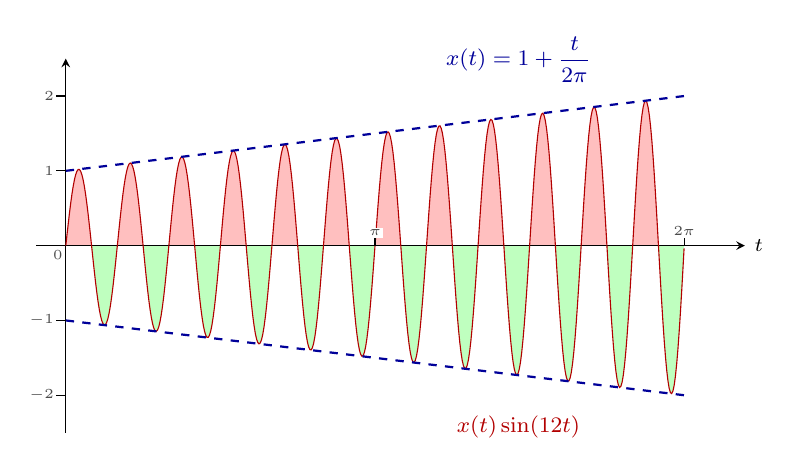
\begin{tikzpicture}[x=1.25cm,y=0.95cm]
  \foreach \k in {0,2,...,22}{%
    \pgfmathsetmacro\a{\k*pi/12}\pgfmathsetmacro\b{(\k+1)*pi/12}%
    \fill[red!25] plot[domain=\a:\b,samples=14] (\x,{(1+\x/(2*pi))*sin(12*\x r)}) -- cycle;}
  \foreach \k in {1,3,...,23}{%
    \pgfmathsetmacro\a{\k*pi/12}\pgfmathsetmacro\b{(\k+1)*pi/12}%
    \fill[green!25] plot[domain=\a:\b,samples=14] (\x,{(1+\x/(2*pi))*sin(12*\x r)}) -- cycle;}
  \taxes{-0.3}{6.9}{2.5}{-2.5}
  \draw[res,thin,domain=0:6.2832,samples=500] plot (\x,{(1+\x/(2*pi))*sin(12*\x r)});
  \draw[sig,dashed,domain=0:6.2832] plot (\x,{1+\x/(2*pi)});
  \draw[sig,dashed,domain=0:6.2832] plot (\x,{-1-\x/(2*pi)});
  \xtu{3.1416}{\pi}\xtu{6.2832}{2\pi}
  \yt{1}{1}\yt{2}{2}\yt{-1}{-1}\yt{-2}{-2}
  \node[font=\footnotesize,blue!60!black,anchor=south] at (4.6,2.05) {$x(t)=1+\dfrac{t}{2\pi}$};
  \node[font=\footnotesize,red!70!black,anchor=north] at (4.6,-2.15) {$x(t)\sin(12t)$};
\end{tikzpicture}
\caption{$x(t)=1+\frac{t}{2\pi}$ 乘以 $\sin(12t)$（$0\le t\le 2\pi$）。虚线是包络 $\pm x(t)$。相邻的红块与绿块面积几乎相等，抵消后只剩一点点；$N$ 越大，剩得越少。}
\end{figure}

\point{数值例子。}取上图的 $x(t)=1+\frac{t}{2\pi}$，在 $[0,2\pi]$ 上分部积分可得（$N$ 为正整数）
\[
\int_0^{2\pi}\Big(1+\frac{t}{2\pi}\Big)\sin(Nt)\,\mathrm{d}t=-\frac{1}{N},\qquad
\int_0^{2\pi}\Big(1+\frac{t}{2\pi}\Big)\cos(Nt)\,\mathrm{d}t=0 .
\]
数值积分的结果：
\begin{center}
\begin{tabular}{ccccc}
\toprule
$N$ & $1$ & $10$ & $100$ & $1000$\\
\midrule
$\int_0^{2\pi}x(t)\sin(Nt)\,\mathrm{d}t$ & $-1.000$ & $-0.100$ & $-0.0100$ & $-0.00100$\\
\bottomrule
\end{tabular}
\end{center}
随 $N$ 增大按 $1/N$ 趋于 $0$。

\point{为什么要条件 \textcircled{\scriptsize 2}：变化不能太剧烈。}若 $x(t)$ 自己也像 $\sin$ 一样无限振荡，两个剧烈振荡的函数相乘，正负块不一定能配对抵消，积分不一定趋于 $0$。条件 \textcircled{\scriptsize 2} 规定一个周期内极值个数有限，等于限制了 $x(t)$ 变化的剧烈程度，保证它相对 $\sin(Nt)$ 是平缓的。

\point{为什么要条件 \textcircled{\scriptsize 1}：不能无限上冲。}若 $x(t)$ 在某点附近无限上冲（不绝对可积），哪怕只差一点点，那里的一块面积也会比相邻的一块大得多，抵消不掉。

\example{不绝对可积时引理一不成立}{极限是 $\pi/2$，不是 $0$}{}
取 $x(t)=\frac{1}{t}$，$0<t\le\pi$。它在 $t\to0^+$ 时无限上冲，$\int_0^{\pi}\frac{\mathrm{d}t}{t}=+\infty$，不绝对可积（但它单调，极值个数有限）。换元 $s=Nt$：
\[
\int_0^{\pi}\frac{\sin(Nt)}{t}\,\mathrm{d}t=\int_0^{N\pi}\frac{\sin s}{s}\,\mathrm{d}s
\ \xrightarrow{\ N\to+\infty\ }\ \int_0^{+\infty}\frac{\sin s}{s}\,\mathrm{d}s=\frac{\pi}{2}\approx1.5708 .
\]
数值：$N=1,10,100,1000$ 时分别为 $1.852$、$1.539$、$1.568$、$1.5705$，确实趋于 $\pi/2$ 而不是 $0$。原因正是 $t=0$ 附近那块正面积：它越来越窄，但越来越高，面积不缩小。

\begin{note}
严格地说，引理一只需要条件 \textcircled{\scriptsize 1}（绝对可积）就成立；条件 \textcircled{\scriptsize 2} 只是让上面的直观解释更容易成立。严格证明较长，见张筑生《数学分析新讲》第二册。
\end{note}

\subsection{引理二：\texorpdfstring{$\sin(\omega t)/t$}{sin(wt)/t} 的积分}\label{sub:lemma2}
\begin{remember}
\[
\int_{-\infty}^{+\infty}\frac{\sin(\omega t)}{t}\,\mathrm{d}t=\pi\qquad(\omega>0).
\]
\end{remember}
换元 $s=\omega t$（$\omega>0$ 时积分限不变）：$\int_{-\infty}^{+\infty}\frac{\sin(\omega t)}{t}\,\mathrm{d}t=\int_{-\infty}^{+\infty}\frac{\sin s}{s}\,\mathrm{d}s$，结果与 $\omega$ 无关。$\frac{\sin s}{s}$ 是偶函数，所以从 $0$ 积到 $+\infty$ 正好是一半 $\frac{\pi}{2}$，上面的例子用到的就是这一半。

\subsection{引理三：\texorpdfstring{$\sin(\omega t)/(\pi t)$}{sin(wt)/(pi t)} 趋于冲激}\label{sub:lemma3}
\begin{remember}
\[
\lim_{\omega\to+\infty}\frac{\sin(\omega t)}{\pi t}=\delta(t).
\]
\end{remember}
理由有三条：
\begin{itemize}[nosep]
\item $t=0$ 处的值为 $\frac{\omega}{\pi}$，$\omega\to+\infty$ 时趋于无穷大；
\item 主瓣在 $t=\pm\frac{\pi}{\omega}$ 处过零，宽度 $\frac{2\pi}{\omega}\to0$；
\item 由引理二，对任意 $\omega>0$，面积 $\int_{-\infty}^{+\infty}\frac{\sin(\omega t)}{\pi t}\,\mathrm{d}t=\frac{\pi}{\pi}=1$，始终不变。
\end{itemize}
又高又窄、面积恒为 $1$，正是冲激函数 $\delta(t)$ 的特征。于是对在 $t=0$ 处连续的函数 $f(t)$，
\[
\lim_{\omega\to+\infty}\int f(t)\,\frac{\sin(\omega t)}{t}\,\mathrm{d}t=\pi\int f(t)\,\delta(t)\,\mathrm{d}t=\pi f(0).
\]

\begin{figure}[H]
\centering
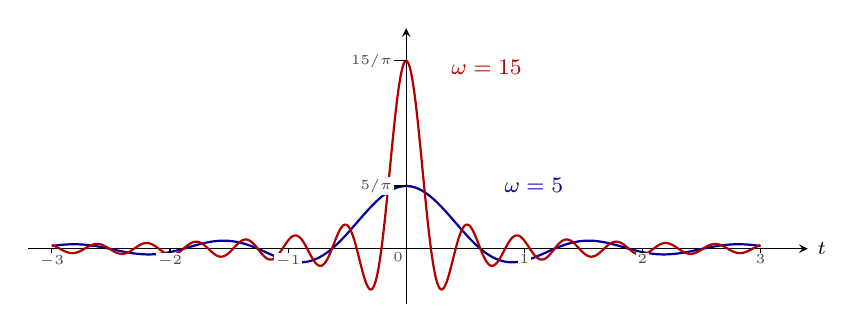
\begin{tikzpicture}[x=1.5cm,y=0.5cm]
  \taxes{-3.2}{3.4}{5.6}{-1.4}
  \draw[sig] plot coordinates {(-3.0000,0.0690) (-2.9900,0.0732) (-2.9800,0.0772) (-2.9700,0.0811) (-2.9600,0.0848) (-2.9500,0.0883) (-2.9400,0.0916) (-2.9300,0.0947) (-2.9200,0.0975) (-2.9100,0.1002) (-2.9000,0.1026) (-2.8900,0.1048) (-2.8800,0.1067) (-2.8700,0.1084) (-2.8600,0.1098) (-2.8500,0.1110) (-2.8400,0.1119) (-2.8300,0.1125) (-2.8200,0.1128) (-2.8100,0.1128) (-2.8000,0.1126) (-2.7900,0.1121) (-2.7800,0.1113) (-2.7700,0.1102) (-2.7600,0.1088) (-2.7500,0.1072) (-2.7400,0.1052) (-2.7300,0.1030) (-2.7200,0.1005) (-2.7100,0.0978) (-2.7000,0.0948) (-2.6900,0.0915) (-2.6800,0.0879) (-2.6700,0.0842) (-2.6600,0.0801) (-2.6500,0.0759) (-2.6400,0.0714) (-2.6300,0.0667) (-2.6200,0.0618) (-2.6100,0.0567) (-2.6000,0.0514) (-2.5900,0.0460) (-2.5800,0.0404) (-2.5700,0.0347) (-2.5600,0.0288) (-2.5500,0.0228) (-2.5400,0.0167) (-2.5300,0.0105) (-2.5200,0.0042) (-2.5100,-0.0021) (-2.5000,-0.0084) (-2.4900,-0.0148) (-2.4800,-0.0213) (-2.4700,-0.0277) (-2.4600,-0.0341) (-2.4500,-0.0404) (-2.4400,-0.0467) (-2.4300,-0.0530) (-2.4200,-0.0591) (-2.4100,-0.0652) (-2.4000,-0.0712) (-2.3900,-0.0770) (-2.3800,-0.0827) (-2.3700,-0.0882) (-2.3600,-0.0935) (-2.3500,-0.0987) (-2.3400,-0.1037) (-2.3300,-0.1084) (-2.3200,-0.1129) (-2.3100,-0.1172) (-2.3000,-0.1212) (-2.2900,-0.1249) (-2.2800,-0.1283) (-2.2700,-0.1315) (-2.2600,-0.1344) (-2.2500,-0.1369) (-2.2400,-0.1391) (-2.2300,-0.1410) (-2.2200,-0.1426) (-2.2100,-0.1438) (-2.2000,-0.1447) (-2.1900,-0.1452) (-2.1800,-0.1453) (-2.1700,-0.1451) (-2.1600,-0.1446) (-2.1500,-0.1436) (-2.1400,-0.1423) (-2.1300,-0.1406) (-2.1200,-0.1386) (-2.1100,-0.1361) (-2.1000,-0.1333) (-2.0900,-0.1302) (-2.0800,-0.1267) (-2.0700,-0.1228) (-2.0600,-0.1186) (-2.0500,-0.1141) (-2.0400,-0.1092) (-2.0300,-0.1040) (-2.0200,-0.0985) (-2.0100,-0.0927) (-2.0000,-0.0866) (-1.9900,-0.0802) (-1.9800,-0.0736) (-1.9700,-0.0667) (-1.9600,-0.0595) (-1.9500,-0.0522) (-1.9400,-0.0446) (-1.9300,-0.0368) (-1.9200,-0.0289) (-1.9100,-0.0208) (-1.9000,-0.0126) (-1.8900,-0.0042) (-1.8800,0.0042) (-1.8700,0.0127) (-1.8600,0.0213) (-1.8500,0.0299) (-1.8400,0.0386) (-1.8300,0.0472) (-1.8200,0.0558) (-1.8100,0.0644) (-1.8000,0.0729) (-1.7900,0.0813) (-1.7800,0.0896) (-1.7700,0.0978) (-1.7600,0.1058) (-1.7500,0.1136) (-1.7400,0.1213) (-1.7300,0.1287) (-1.7200,0.1359) (-1.7100,0.1428) (-1.7000,0.1495) (-1.6900,0.1559) (-1.6800,0.1619) (-1.6700,0.1676) (-1.6600,0.1730) (-1.6500,0.1780) (-1.6400,0.1826) (-1.6300,0.1868) (-1.6200,0.1906) (-1.6100,0.1939) (-1.6000,0.1968) (-1.5900,0.1993) (-1.5800,0.2012) (-1.5700,0.2027) (-1.5600,0.2037) (-1.5500,0.2043) (-1.5400,0.2042) (-1.5300,0.2037) (-1.5200,0.2027) (-1.5100,0.2011) (-1.5000,0.1990) (-1.4900,0.1964) (-1.4800,0.1933) (-1.4700,0.1896) (-1.4600,0.1854) (-1.4500,0.1807) (-1.4400,0.1754) (-1.4300,0.1697) (-1.4200,0.1634) (-1.4100,0.1566) (-1.4000,0.1494) (-1.3900,0.1416) (-1.3800,0.1334) (-1.3700,0.1248) (-1.3600,0.1156) (-1.3500,0.1061) (-1.3400,0.0962) (-1.3300,0.0858) (-1.3200,0.0751) (-1.3100,0.0641) (-1.3000,0.0527) (-1.2900,0.0410) (-1.2800,0.0290) (-1.2700,0.0167) (-1.2600,0.0042) (-1.2500,-0.0084) (-1.2400,-0.0213) (-1.2300,-0.0344) (-1.2200,-0.0475) (-1.2100,-0.0608) (-1.2000,-0.0741) (-1.1900,-0.0875) (-1.1800,-0.1009) (-1.1700,-0.1142) (-1.1600,-0.1275) (-1.1500,-0.1407) (-1.1400,-0.1538) (-1.1300,-0.1667) (-1.1200,-0.1794) (-1.1100,-0.1919) (-1.1000,-0.2042) (-1.0900,-0.2161) (-1.0800,-0.2278) (-1.0700,-0.2390) (-1.0600,-0.2499) (-1.0500,-0.2604) (-1.0400,-0.2704) (-1.0300,-0.2799) (-1.0200,-0.2889) (-1.0100,-0.2974) (-1.0000,-0.3052) (-0.9900,-0.3125) (-0.9800,-0.3191) (-0.9700,-0.3251) (-0.9600,-0.3303) (-0.9500,-0.3348) (-0.9400,-0.3386) (-0.9300,-0.3416) (-0.9200,-0.3438) (-0.9100,-0.3452) (-0.9000,-0.3457) (-0.8900,-0.3454) (-0.8800,-0.3442) (-0.8700,-0.3421) (-0.8600,-0.3391) (-0.8500,-0.3352) (-0.8400,-0.3303) (-0.8300,-0.3244) (-0.8200,-0.3176) (-0.8100,-0.3099) (-0.8000,-0.3011) (-0.7900,-0.2914) (-0.7800,-0.2807) (-0.7700,-0.2690) (-0.7600,-0.2563) (-0.7500,-0.2426) (-0.7400,-0.2279) (-0.7300,-0.2123) (-0.7200,-0.1956) (-0.7100,-0.1781) (-0.7000,-0.1595) (-0.6900,-0.1400) (-0.6800,-0.1196) (-0.6700,-0.0983) (-0.6600,-0.0761) (-0.6500,-0.0530) (-0.6400,-0.0290) (-0.6300,-0.0042) (-0.6200,0.0213) (-0.6100,0.0477) (-0.6000,0.0749) (-0.5900,0.1027) (-0.5800,0.1313) (-0.5700,0.1605) (-0.5600,0.1904) (-0.5500,0.2209) (-0.5400,0.2519) (-0.5300,0.2835) (-0.5200,0.3156) (-0.5100,0.3481) (-0.5000,0.3810) (-0.4900,0.4143) (-0.4800,0.4479) (-0.4700,0.4818) (-0.4600,0.5160) (-0.4500,0.5504) (-0.4400,0.5849) (-0.4300,0.6195) (-0.4200,0.6542) (-0.4100,0.6889) (-0.4000,0.7236) (-0.3900,0.7582) (-0.3800,0.7927) (-0.3700,0.8270) (-0.3600,0.8611) (-0.3500,0.8949) (-0.3400,0.9284) (-0.3300,0.9616) (-0.3200,0.9943) (-0.3100,1.0266) (-0.3000,1.0584) (-0.2900,1.0896) (-0.2800,1.1203) (-0.2700,1.1503) (-0.2600,1.1797) (-0.2500,1.2083) (-0.2400,1.2362) (-0.2300,1.2632) (-0.2200,1.2895) (-0.2100,1.3148) (-0.2000,1.3392) (-0.1900,1.3627) (-0.1800,1.3852) (-0.1700,1.4067) (-0.1600,1.4271) (-0.1500,1.4465) (-0.1400,1.4647) (-0.1300,1.4818) (-0.1200,1.4978) (-0.1100,1.5125) (-0.1000,1.5261) (-0.0900,1.5384) (-0.0800,1.5494) (-0.0700,1.5593) (-0.0600,1.5678) (-0.0500,1.5750) (-0.0400,1.5810) (-0.0300,1.5856) (-0.0200,1.5889) (-0.0100,1.5909) (0.0000,1.5915) (0.0100,1.5909) (0.0200,1.5889) (0.0300,1.5856) (0.0400,1.5810) (0.0500,1.5750) (0.0600,1.5678) (0.0700,1.5593) (0.0800,1.5494) (0.0900,1.5384) (0.1000,1.5261) (0.1100,1.5125) (0.1200,1.4978) (0.1300,1.4818) (0.1400,1.4647) (0.1500,1.4465) (0.1600,1.4271) (0.1700,1.4067) (0.1800,1.3852) (0.1900,1.3627) (0.2000,1.3392) (0.2100,1.3148) (0.2200,1.2895) (0.2300,1.2632) (0.2400,1.2362) (0.2500,1.2083) (0.2600,1.1797) (0.2700,1.1503) (0.2800,1.1203) (0.2900,1.0896) (0.3000,1.0584) (0.3100,1.0266) (0.3200,0.9943) (0.3300,0.9616) (0.3400,0.9284) (0.3500,0.8949) (0.3600,0.8611) (0.3700,0.8270) (0.3800,0.7927) (0.3900,0.7582) (0.4000,0.7236) (0.4100,0.6889) (0.4200,0.6542) (0.4300,0.6195) (0.4400,0.5849) (0.4500,0.5504) (0.4600,0.5160) (0.4700,0.4818) (0.4800,0.4479) (0.4900,0.4143) (0.5000,0.3810) (0.5100,0.3481) (0.5200,0.3156) (0.5300,0.2835) (0.5400,0.2519) (0.5500,0.2209) (0.5600,0.1904) (0.5700,0.1605) (0.5800,0.1313) (0.5900,0.1027) (0.6000,0.0749) (0.6100,0.0477) (0.6200,0.0213) (0.6300,-0.0042) (0.6400,-0.0290) (0.6500,-0.0530) (0.6600,-0.0761) (0.6700,-0.0983) (0.6800,-0.1196) (0.6900,-0.1400) (0.7000,-0.1595) (0.7100,-0.1781) (0.7200,-0.1956) (0.7300,-0.2123) (0.7400,-0.2279) (0.7500,-0.2426) (0.7600,-0.2563) (0.7700,-0.2690) (0.7800,-0.2807) (0.7900,-0.2914) (0.8000,-0.3011) (0.8100,-0.3099) (0.8200,-0.3176) (0.8300,-0.3244) (0.8400,-0.3303) (0.8500,-0.3352) (0.8600,-0.3391) (0.8700,-0.3421) (0.8800,-0.3442) (0.8900,-0.3454) (0.9000,-0.3457) (0.9100,-0.3452) (0.9200,-0.3438) (0.9300,-0.3416) (0.9400,-0.3386) (0.9500,-0.3348) (0.9600,-0.3303) (0.9700,-0.3251) (0.9800,-0.3191) (0.9900,-0.3125) (1.0000,-0.3052) (1.0100,-0.2974) (1.0200,-0.2889) (1.0300,-0.2799) (1.0400,-0.2704) (1.0500,-0.2604) (1.0600,-0.2499) (1.0700,-0.2390) (1.0800,-0.2278) (1.0900,-0.2161) (1.1000,-0.2042) (1.1100,-0.1919) (1.1200,-0.1794) (1.1300,-0.1667) (1.1400,-0.1538) (1.1500,-0.1407) (1.1600,-0.1275) (1.1700,-0.1142) (1.1800,-0.1009) (1.1900,-0.0875) (1.2000,-0.0741) (1.2100,-0.0608) (1.2200,-0.0475) (1.2300,-0.0344) (1.2400,-0.0213) (1.2500,-0.0084) (1.2600,0.0042) (1.2700,0.0167) (1.2800,0.0290) (1.2900,0.0410) (1.3000,0.0527) (1.3100,0.0641) (1.3200,0.0751) (1.3300,0.0858) (1.3400,0.0962) (1.3500,0.1061) (1.3600,0.1156) (1.3700,0.1248) (1.3800,0.1334) (1.3900,0.1416) (1.4000,0.1494) (1.4100,0.1566) (1.4200,0.1634) (1.4300,0.1697) (1.4400,0.1754) (1.4500,0.1807) (1.4600,0.1854) (1.4700,0.1896) (1.4800,0.1933) (1.4900,0.1964) (1.5000,0.1990) (1.5100,0.2011) (1.5200,0.2027) (1.5300,0.2037) (1.5400,0.2042) (1.5500,0.2043) (1.5600,0.2037) (1.5700,0.2027) (1.5800,0.2012) (1.5900,0.1993) (1.6000,0.1968) (1.6100,0.1939) (1.6200,0.1906) (1.6300,0.1868) (1.6400,0.1826) (1.6500,0.1780) (1.6600,0.1730) (1.6700,0.1676) (1.6800,0.1619) (1.6900,0.1559) (1.7000,0.1495) (1.7100,0.1428) (1.7200,0.1359) (1.7300,0.1287) (1.7400,0.1213) (1.7500,0.1136) (1.7600,0.1058) (1.7700,0.0978) (1.7800,0.0896) (1.7900,0.0813) (1.8000,0.0729) (1.8100,0.0644) (1.8200,0.0558) (1.8300,0.0472) (1.8400,0.0386) (1.8500,0.0299) (1.8600,0.0213) (1.8700,0.0127) (1.8800,0.0042) (1.8900,-0.0042) (1.9000,-0.0126) (1.9100,-0.0208) (1.9200,-0.0289) (1.9300,-0.0368) (1.9400,-0.0446) (1.9500,-0.0522) (1.9600,-0.0595) (1.9700,-0.0667) (1.9800,-0.0736) (1.9900,-0.0802) (2.0000,-0.0866) (2.0100,-0.0927) (2.0200,-0.0985) (2.0300,-0.1040) (2.0400,-0.1092) (2.0500,-0.1141) (2.0600,-0.1186) (2.0700,-0.1228) (2.0800,-0.1267) (2.0900,-0.1302) (2.1000,-0.1333) (2.1100,-0.1361) (2.1200,-0.1386) (2.1300,-0.1406) (2.1400,-0.1423) (2.1500,-0.1436) (2.1600,-0.1446) (2.1700,-0.1451) (2.1800,-0.1453) (2.1900,-0.1452) (2.2000,-0.1447) (2.2100,-0.1438) (2.2200,-0.1426) (2.2300,-0.1410) (2.2400,-0.1391) (2.2500,-0.1369) (2.2600,-0.1344) (2.2700,-0.1315) (2.2800,-0.1283) (2.2900,-0.1249) (2.3000,-0.1212) (2.3100,-0.1172) (2.3200,-0.1129) (2.3300,-0.1084) (2.3400,-0.1037) (2.3500,-0.0987) (2.3600,-0.0935) (2.3700,-0.0882) (2.3800,-0.0827) (2.3900,-0.0770) (2.4000,-0.0712) (2.4100,-0.0652) (2.4200,-0.0591) (2.4300,-0.0530) (2.4400,-0.0467) (2.4500,-0.0404) (2.4600,-0.0341) (2.4700,-0.0277) (2.4800,-0.0213) (2.4900,-0.0148) (2.5000,-0.0084) (2.5100,-0.0021) (2.5200,0.0042) (2.5300,0.0105) (2.5400,0.0167) (2.5500,0.0228) (2.5600,0.0288) (2.5700,0.0347) (2.5800,0.0404) (2.5900,0.0460) (2.6000,0.0514) (2.6100,0.0567) (2.6200,0.0618) (2.6300,0.0667) (2.6400,0.0714) (2.6500,0.0759) (2.6600,0.0801) (2.6700,0.0842) (2.6800,0.0879) (2.6900,0.0915) (2.7000,0.0948) (2.7100,0.0978) (2.7200,0.1005) (2.7300,0.1030) (2.7400,0.1052) (2.7500,0.1072) (2.7600,0.1088) (2.7700,0.1102) (2.7800,0.1113) (2.7900,0.1121) (2.8000,0.1126) (2.8100,0.1128) (2.8200,0.1128) (2.8300,0.1125) (2.8400,0.1119) (2.8500,0.1110) (2.8600,0.1098) (2.8700,0.1084) (2.8800,0.1067) (2.8900,0.1048) (2.9000,0.1026) (2.9100,0.1002) (2.9200,0.0975) (2.9300,0.0947) (2.9400,0.0916) (2.9500,0.0883) (2.9600,0.0848) (2.9700,0.0811) (2.9800,0.0772) (2.9900,0.0732) (3.0000,0.0690)};
  \draw[res] plot coordinates {(-3.0000,0.0903) (-2.9900,0.0812) (-2.9800,0.0702) (-2.9700,0.0576) (-2.9600,0.0436) (-2.9500,0.0285) (-2.9400,0.0127) (-2.9300,-0.0035) (-2.9200,-0.0198) (-2.9100,-0.0357) (-2.9000,-0.0509) (-2.8900,-0.0651) (-2.8800,-0.0779) (-2.8700,-0.0891) (-2.8600,-0.0983) (-2.8500,-0.1053) (-2.8400,-0.1101) (-2.8300,-0.1124) (-2.8200,-0.1122) (-2.8100,-0.1094) (-2.8000,-0.1042) (-2.7900,-0.0966) (-2.7800,-0.0867) (-2.7700,-0.0748) (-2.7600,-0.0612) (-2.7500,-0.0461) (-2.7400,-0.0298) (-2.7300,-0.0127) (-2.7200,0.0048) (-2.7100,0.0223) (-2.7000,0.0394) (-2.6900,0.0558) (-2.6800,0.0710) (-2.6700,0.0847) (-2.6600,0.0967) (-2.6500,0.1065) (-2.6400,0.1141) (-2.6300,0.1191) (-2.6200,0.1214) (-2.6100,0.1211) (-2.6000,0.1180) (-2.5900,0.1122) (-2.5800,0.1039) (-2.5700,0.0931) (-2.5600,0.0802) (-2.5500,0.0653) (-2.5400,0.0489) (-2.5300,0.0312) (-2.5200,0.0127) (-2.5100,-0.0062) (-2.5000,-0.0252) (-2.4900,-0.0437) (-2.4800,-0.0614) (-2.4700,-0.0779) (-2.4600,-0.0927) (-2.4500,-0.1056) (-2.4400,-0.1162) (-2.4300,-0.1243) (-2.4200,-0.1296) (-2.4100,-0.1320) (-2.4000,-0.1315) (-2.3900,-0.1281) (-2.3800,-0.1217) (-2.3700,-0.1125) (-2.3600,-0.1007) (-2.3500,-0.0865) (-2.3400,-0.0702) (-2.3300,-0.0523) (-2.3200,-0.0329) (-2.3100,-0.0127) (-2.3000,0.0080) (-2.2900,0.0286) (-2.2800,0.0489) (-2.2700,0.0682) (-2.2600,0.0861) (-2.2500,0.1022) (-2.2400,0.1162) (-2.2300,0.1277) (-2.2200,0.1364) (-2.2100,0.1421) (-2.2000,0.1447) (-2.1900,0.1440) (-2.1800,0.1401) (-2.1700,0.1329) (-2.1600,0.1227) (-2.1500,0.1097) (-2.1400,0.0940) (-2.1300,0.0761) (-2.1200,0.0563) (-2.1100,0.0350) (-2.1000,0.0127) (-2.0900,-0.0100) (-2.0800,-0.0328) (-2.0700,-0.0550) (-2.0600,-0.0762) (-2.0500,-0.0959) (-2.0400,-0.1136) (-2.0300,-0.1290) (-2.0200,-0.1416) (-2.0100,-0.1511) (-2.0000,-0.1573) (-1.9900,-0.1600) (-1.9800,-0.1591) (-1.9700,-0.1546) (-1.9600,-0.1466) (-1.9500,-0.1352) (-1.9400,-0.1206) (-1.9300,-0.1031) (-1.9200,-0.0832) (-1.9100,-0.0611) (-1.9000,-0.0375) (-1.8900,-0.0127) (-1.8800,0.0126) (-1.8700,0.0379) (-1.8600,0.0626) (-1.8500,0.0861) (-1.8400,0.1080) (-1.8300,0.1277) (-1.8200,0.1447) (-1.8100,0.1586) (-1.8000,0.1691) (-1.7900,0.1759) (-1.7800,0.1788) (-1.7700,0.1777) (-1.7600,0.1726) (-1.7500,0.1635) (-1.7400,0.1506) (-1.7300,0.1342) (-1.7200,0.1145) (-1.7100,0.0920) (-1.7000,0.0672) (-1.6900,0.0406) (-1.6800,0.0127) (-1.6700,-0.0158) (-1.6600,-0.0442) (-1.6500,-0.0720) (-1.6400,-0.0986) (-1.6300,-0.1232) (-1.6200,-0.1454) (-1.6100,-0.1645) (-1.6000,-0.1802) (-1.5900,-0.1919) (-1.5800,-0.1995) (-1.5700,-0.2027) (-1.5600,-0.2014) (-1.5500,-0.1955) (-1.5400,-0.1850) (-1.5300,-0.1703) (-1.5200,-0.1515) (-1.5100,-0.1291) (-1.5000,-0.1034) (-1.4900,-0.0750) (-1.4800,-0.0446) (-1.4700,-0.0127) (-1.4600,0.0198) (-1.4500,0.0524) (-1.4400,0.0843) (-1.4300,0.1147) (-1.4200,0.1429) (-1.4100,0.1683) (-1.4000,0.1902) (-1.3900,0.2082) (-1.3800,0.2217) (-1.3700,0.2304) (-1.3600,0.2340) (-1.3500,0.2324) (-1.3400,0.2255) (-1.3300,0.2133) (-1.3200,0.1962) (-1.3100,0.1744) (-1.3000,0.1483) (-1.2900,0.1184) (-1.2800,0.0854) (-1.2700,0.0499) (-1.2600,0.0127) (-1.2500,-0.0253) (-1.2400,-0.0634) (-1.2300,-0.1007) (-1.2200,-0.1363) (-1.2100,-0.1694) (-1.2000,-0.1992) (-1.1900,-0.2250) (-1.1800,-0.2462) (-1.1700,-0.2621) (-1.1600,-0.2724) (-1.1500,-0.2767) (-1.1400,-0.2748) (-1.1300,-0.2666) (-1.1200,-0.2523) (-1.1100,-0.2319) (-1.1000,-0.2060) (-1.0900,-0.1749) (-1.0800,-0.1392) (-1.0700,-0.0998) (-1.0600,-0.0573) (-1.0500,-0.0127) (-1.0400,0.0330) (-1.0300,0.0788) (-1.0200,0.1238) (-1.0100,0.1669) (-1.0000,0.2070) (-0.9900,0.2432) (-0.9800,0.2747) (-0.9700,0.3006) (-0.9600,0.3202) (-0.9500,0.3329) (-0.9400,0.3384) (-0.9300,0.3363) (-0.9200,0.3265) (-0.9100,0.3091) (-0.9000,0.2843) (-0.8900,0.2525) (-0.8800,0.2142) (-0.8700,0.1701) (-0.8600,0.1212) (-0.8500,0.0684) (-0.8400,0.0127) (-0.8300,-0.0445) (-0.8200,-0.1022) (-0.8100,-0.1589) (-0.8000,-0.2135) (-0.7900,-0.2646) (-0.7800,-0.3110) (-0.7700,-0.3515) (-0.7600,-0.3850) (-0.7500,-0.4108) (-0.7400,-0.4278) (-0.7300,-0.4356) (-0.7200,-0.4337) (-0.7100,-0.4218) (-0.7000,-0.4000) (-0.6900,-0.3685) (-0.6800,-0.3276) (-0.6700,-0.2781) (-0.6600,-0.2207) (-0.6500,-0.1565) (-0.6400,-0.0867) (-0.6300,-0.0127) (-0.6200,0.0639) (-0.6100,0.1416) (-0.6000,0.2186) (-0.5900,0.2933) (-0.5800,0.3638) (-0.5700,0.4285) (-0.5600,0.4858) (-0.5500,0.5340) (-0.5400,0.5717) (-0.5300,0.5978) (-0.5200,0.6112) (-0.5100,0.6112) (-0.5000,0.5971) (-0.4900,0.5688) (-0.4800,0.5263) (-0.4700,0.4699) (-0.4600,0.4003) (-0.4500,0.3183) (-0.4400,0.2254) (-0.4300,0.1229) (-0.4200,0.0127) (-0.4100,-0.1031) (-0.4000,-0.2224) (-0.3900,-0.3426) (-0.3800,-0.4613) (-0.3700,-0.5757) (-0.3600,-0.6833) (-0.3500,-0.7812) (-0.3400,-0.8668) (-0.3300,-0.9375) (-0.3200,-0.9909) (-0.3100,-1.0248) (-0.3000,-1.0372) (-0.2900,-1.0263) (-0.2800,-0.9908) (-0.2700,-0.9296) (-0.2600,-0.8420) (-0.2500,-0.7277) (-0.2400,-0.5869) (-0.2300,-0.4201) (-0.2200,-0.2282) (-0.2100,-0.0127) (-0.2000,0.2246) (-0.1900,0.4816) (-0.1800,0.7558) (-0.1700,1.0442) (-0.1600,1.3438) (-0.1500,1.6511) (-0.1400,1.9626) (-0.1300,2.2746) (-0.1200,2.5832) (-0.1100,2.8847) (-0.1000,3.1751) (-0.0900,3.4509) (-0.0800,3.7085) (-0.0700,3.9444) (-0.0600,4.1557) (-0.0500,4.3394) (-0.0400,4.4933) (-0.0300,4.6151) (-0.0200,4.7034) (-0.0100,4.7568) (0.0000,4.7746) (0.0100,4.7568) (0.0200,4.7034) (0.0300,4.6151) (0.0400,4.4933) (0.0500,4.3394) (0.0600,4.1557) (0.0700,3.9444) (0.0800,3.7085) (0.0900,3.4509) (0.1000,3.1751) (0.1100,2.8847) (0.1200,2.5832) (0.1300,2.2746) (0.1400,1.9626) (0.1500,1.6511) (0.1600,1.3438) (0.1700,1.0442) (0.1800,0.7558) (0.1900,0.4816) (0.2000,0.2246) (0.2100,-0.0127) (0.2200,-0.2282) (0.2300,-0.4201) (0.2400,-0.5869) (0.2500,-0.7277) (0.2600,-0.8420) (0.2700,-0.9296) (0.2800,-0.9908) (0.2900,-1.0263) (0.3000,-1.0372) (0.3100,-1.0248) (0.3200,-0.9909) (0.3300,-0.9375) (0.3400,-0.8668) (0.3500,-0.7812) (0.3600,-0.6833) (0.3700,-0.5757) (0.3800,-0.4613) (0.3900,-0.3426) (0.4000,-0.2224) (0.4100,-0.1031) (0.4200,0.0127) (0.4300,0.1229) (0.4400,0.2254) (0.4500,0.3183) (0.4600,0.4003) (0.4700,0.4699) (0.4800,0.5263) (0.4900,0.5688) (0.5000,0.5971) (0.5100,0.6112) (0.5200,0.6112) (0.5300,0.5978) (0.5400,0.5717) (0.5500,0.5340) (0.5600,0.4858) (0.5700,0.4285) (0.5800,0.3638) (0.5900,0.2933) (0.6000,0.2186) (0.6100,0.1416) (0.6200,0.0639) (0.6300,-0.0127) (0.6400,-0.0867) (0.6500,-0.1565) (0.6600,-0.2207) (0.6700,-0.2781) (0.6800,-0.3276) (0.6900,-0.3685) (0.7000,-0.4000) (0.7100,-0.4218) (0.7200,-0.4337) (0.7300,-0.4356) (0.7400,-0.4278) (0.7500,-0.4108) (0.7600,-0.3850) (0.7700,-0.3515) (0.7800,-0.3110) (0.7900,-0.2646) (0.8000,-0.2135) (0.8100,-0.1589) (0.8200,-0.1022) (0.8300,-0.0445) (0.8400,0.0127) (0.8500,0.0684) (0.8600,0.1212) (0.8700,0.1701) (0.8800,0.2142) (0.8900,0.2525) (0.9000,0.2843) (0.9100,0.3091) (0.9200,0.3265) (0.9300,0.3363) (0.9400,0.3384) (0.9500,0.3329) (0.9600,0.3202) (0.9700,0.3006) (0.9800,0.2747) (0.9900,0.2432) (1.0000,0.2070) (1.0100,0.1669) (1.0200,0.1238) (1.0300,0.0788) (1.0400,0.0330) (1.0500,-0.0127) (1.0600,-0.0573) (1.0700,-0.0998) (1.0800,-0.1392) (1.0900,-0.1749) (1.1000,-0.2060) (1.1100,-0.2319) (1.1200,-0.2523) (1.1300,-0.2666) (1.1400,-0.2748) (1.1500,-0.2767) (1.1600,-0.2724) (1.1700,-0.2621) (1.1800,-0.2462) (1.1900,-0.2250) (1.2000,-0.1992) (1.2100,-0.1694) (1.2200,-0.1363) (1.2300,-0.1007) (1.2400,-0.0634) (1.2500,-0.0253) (1.2600,0.0127) (1.2700,0.0499) (1.2800,0.0854) (1.2900,0.1184) (1.3000,0.1483) (1.3100,0.1744) (1.3200,0.1962) (1.3300,0.2133) (1.3400,0.2255) (1.3500,0.2324) (1.3600,0.2340) (1.3700,0.2304) (1.3800,0.2217) (1.3900,0.2082) (1.4000,0.1902) (1.4100,0.1683) (1.4200,0.1429) (1.4300,0.1147) (1.4400,0.0843) (1.4500,0.0524) (1.4600,0.0198) (1.4700,-0.0127) (1.4800,-0.0446) (1.4900,-0.0750) (1.5000,-0.1034) (1.5100,-0.1291) (1.5200,-0.1515) (1.5300,-0.1703) (1.5400,-0.1850) (1.5500,-0.1955) (1.5600,-0.2014) (1.5700,-0.2027) (1.5800,-0.1995) (1.5900,-0.1919) (1.6000,-0.1802) (1.6100,-0.1645) (1.6200,-0.1454) (1.6300,-0.1232) (1.6400,-0.0986) (1.6500,-0.0720) (1.6600,-0.0442) (1.6700,-0.0158) (1.6800,0.0127) (1.6900,0.0406) (1.7000,0.0672) (1.7100,0.0920) (1.7200,0.1145) (1.7300,0.1342) (1.7400,0.1506) (1.7500,0.1635) (1.7600,0.1726) (1.7700,0.1777) (1.7800,0.1788) (1.7900,0.1759) (1.8000,0.1691) (1.8100,0.1586) (1.8200,0.1447) (1.8300,0.1277) (1.8400,0.1080) (1.8500,0.0861) (1.8600,0.0626) (1.8700,0.0379) (1.8800,0.0126) (1.8900,-0.0127) (1.9000,-0.0375) (1.9100,-0.0611) (1.9200,-0.0832) (1.9300,-0.1031) (1.9400,-0.1206) (1.9500,-0.1352) (1.9600,-0.1466) (1.9700,-0.1546) (1.9800,-0.1591) (1.9900,-0.1600) (2.0000,-0.1573) (2.0100,-0.1511) (2.0200,-0.1416) (2.0300,-0.1290) (2.0400,-0.1136) (2.0500,-0.0959) (2.0600,-0.0762) (2.0700,-0.0550) (2.0800,-0.0328) (2.0900,-0.0100) (2.1000,0.0127) (2.1100,0.0350) (2.1200,0.0563) (2.1300,0.0761) (2.1400,0.0940) (2.1500,0.1097) (2.1600,0.1227) (2.1700,0.1329) (2.1800,0.1401) (2.1900,0.1440) (2.2000,0.1447) (2.2100,0.1421) (2.2200,0.1364) (2.2300,0.1277) (2.2400,0.1162) (2.2500,0.1022) (2.2600,0.0861) (2.2700,0.0682) (2.2800,0.0489) (2.2900,0.0286) (2.3000,0.0080) (2.3100,-0.0127) (2.3200,-0.0329) (2.3300,-0.0523) (2.3400,-0.0702) (2.3500,-0.0865) (2.3600,-0.1007) (2.3700,-0.1125) (2.3800,-0.1217) (2.3900,-0.1281) (2.4000,-0.1315) (2.4100,-0.1320) (2.4200,-0.1296) (2.4300,-0.1243) (2.4400,-0.1162) (2.4500,-0.1056) (2.4600,-0.0927) (2.4700,-0.0779) (2.4800,-0.0614) (2.4900,-0.0437) (2.5000,-0.0252) (2.5100,-0.0062) (2.5200,0.0127) (2.5300,0.0312) (2.5400,0.0489) (2.5500,0.0653) (2.5600,0.0802) (2.5700,0.0931) (2.5800,0.1039) (2.5900,0.1122) (2.6000,0.1180) (2.6100,0.1211) (2.6200,0.1214) (2.6300,0.1191) (2.6400,0.1141) (2.6500,0.1065) (2.6600,0.0967) (2.6700,0.0847) (2.6800,0.0710) (2.6900,0.0558) (2.7000,0.0394) (2.7100,0.0223) (2.7200,0.0048) (2.7300,-0.0127) (2.7400,-0.0298) (2.7500,-0.0461) (2.7600,-0.0612) (2.7700,-0.0748) (2.7800,-0.0867) (2.7900,-0.0966) (2.8000,-0.1042) (2.8100,-0.1094) (2.8200,-0.1122) (2.8300,-0.1124) (2.8400,-0.1101) (2.8500,-0.1053) (2.8600,-0.0983) (2.8700,-0.0891) (2.8800,-0.0779) (2.8900,-0.0651) (2.9000,-0.0509) (2.9100,-0.0357) (2.9200,-0.0198) (2.9300,-0.0035) (2.9400,0.0127) (2.9500,0.0285) (2.9600,0.0436) (2.9700,0.0576) (2.9800,0.0702) (2.9900,0.0812) (3.0000,0.0903)};
  \xt{-3}{-3}\xt{-2}{-2}\xt{-1}{-1}\xt{1}{1}\xt{2}{2}\xt{3}{3}
  \yt{1.5915}{5/\pi}\yt{4.7746}{15/\pi}
  \node[font=\footnotesize,blue!60!black,anchor=west] at (0.75,1.6) {$\omega=5$};
  \node[font=\footnotesize,red!70!black,anchor=west] at (0.3,4.6) {$\omega=15$};
\end{tikzpicture}
\caption{$\frac{\sin(\omega t)}{\pi t}$ 在 $\omega=5$（蓝）和 $\omega=15$（红）时的形状。$\omega$ 越大，峰越高（$\frac{\omega}{\pi}$）、主瓣越窄（$\frac{2\pi}{\omega}$），曲线下的面积始终为 $1$，趋于 $\delta(t)$。}
\end{figure}

%==================================================================
\section{证明}\label{sec:proof}

\subsection{第一步：代入系数，合并成一个积分}
把 $B_0$、$B_k$、$C_k$ 代入 $X_N(t)$：
\begin{align*}
X_N(t)&=\frac{1}{T_0}\int_{T_0}x(u)\,\mathrm{d}u
+\frac{2}{T_0}\sum_{k=1}^{N}\Big[\int_{T_0}x(u)\cos(k\omega_0u)\,\mathrm{d}u\Big]\cos(k\omega_0t)\\
&\quad+\frac{2}{T_0}\sum_{k=1}^{N}\Big[\int_{T_0}x(u)\sin(k\omega_0u)\,\mathrm{d}u\Big]\sin(k\omega_0t).
\end{align*}
$\cos(k\omega_0t)$、$\sin(k\omega_0t)$ 与积分变量 $u$ 无关，可以放进积分里；有限项求和与积分可以交换次序。把三项都写成 $\frac{2}{T_0}\int_{T_0}[\cdots]\,x(u)\,\mathrm{d}u$ 的形式（第一项的系数 $\frac{1}{T_0}=\frac{2}{T_0}\cdot\frac12$）：
\[
X_N(t)=\frac{2}{T_0}\int_{T_0}\Big[\frac12+\sum_{k=1}^{N}\big(\cos(k\omega_0u)\cos(k\omega_0t)+\sin(k\omega_0u)\sin(k\omega_0t)\big)\Big]x(u)\,\mathrm{d}u .
\]
再用 $\cos A\cos B+\sin A\sin B=\cos(A-B)$：
\[
X_N(t)=\frac{2}{T_0}\int_{T_0}\Big[\frac12+\sum_{k=1}^{N}\cos\big(k\omega_0(u-t)\big)\Big]x(u)\,\mathrm{d}u .
\]

\subsection{第二步：把余弦和化成一个分式}\label{sub:kernel}
\begin{remember}
对任意正整数 $N$，
\[
1+2\cos w+2\cos 2w+\cdots+2\cos Nw=\frac{\sin\!\big((N+\frac12)w\big)}{\sin\frac{w}{2}} .
\]
（$\sin\frac w2=0$ 时右边取极限，等于 $2N+1$，与左边一致。）
\end{remember}

\point{证明。}两边同乘 $\sin\frac w2$。左边第一项是 $\sin\frac w2$；其余每项用积化和差
\[
2\cos(kw)\sin\frac w2=\sin\!\Big(kw+\frac w2\Big)-\sin\!\Big(kw-\frac w2\Big)=\sin\!\Big(\big(k+\tfrac12\big)w\Big)-\sin\!\Big(\big(k-\tfrac12\big)w\Big).
\]
于是
\begin{align*}
\sin\frac w2\,\Big[1+2\sum_{k=1}^{N}\cos(kw)\Big]
&=\sin\frac12w+\Big(\sin\frac32w-\sin\frac12w\Big)+\Big(\sin\frac52w-\sin\frac32w\Big)+\cdots\\
&\quad+\Big(\sin\big(N+\tfrac12\big)w-\sin\big(N-\tfrac12\big)w\Big).
\end{align*}
前后相邻的项两两抵消，最后只剩 $\sin\big((N+\frac12)w\big)$。两边再除以 $\sin\frac w2$ 即得。

\point{代回去。}恒等式两边除以 $2$：$\frac12+\sum_{k=1}^{N}\cos(kw)=\frac{\sin((N+\frac12)w)}{2\sin\frac w2}$。取 $w=\omega_0(u-t)$，并把一个周期取成 $[0,T_0]$：
\[
X_N(t)=\frac{1}{T_0}\int_{0}^{T_0}\frac{\sin\!\big((N+\frac12)\,\omega_0(u-t)\big)}{\sin\!\big(\frac12\,\omega_0(u-t)\big)}\,x(u)\,\mathrm{d}u .
\]

\point{狄利克雷核。}这里出现的函数
\[
D_N(u)=\frac{\sin\!\big((N+\frac12)u\big)}{2\sin\frac u2}=\frac12+\sum_{k=1}^{N}\cos(ku)
\]
叫狄利克雷核(Dirichlet kernel)。它有两个性质，后面要用：
\begin{itemize}[nosep]
\item $u=0$ 处的值为 $N+\frac12$，$N$ 越大峰越高、越窄；
\item 在一个周期上的积分恒为 $\pi$：$\int_{-\pi}^{\pi}D_N(u)\,\mathrm{d}u=\int_{-\pi}^{\pi}\frac12\,\mathrm{d}u+\sum_{k=1}^{N}\int_{-\pi}^{\pi}\cos(ku)\,\mathrm{d}u=\pi+0=\pi$。
\end{itemize}

\begin{figure}[H]
\centering
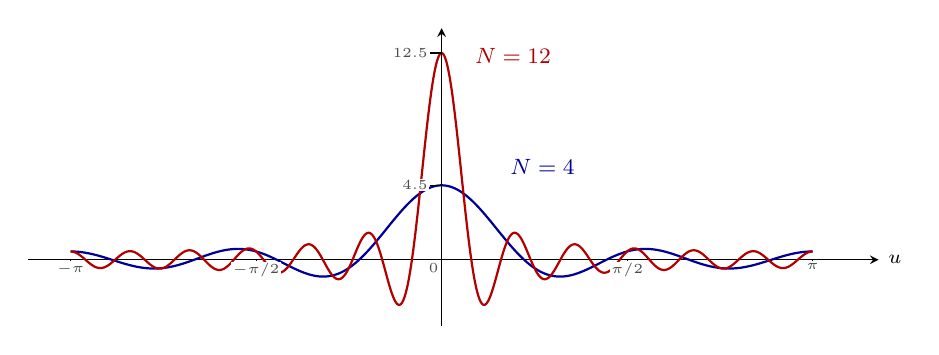
\begin{tikzpicture}[x=1.5cm,y=0.21cm]
  \taxes[u]{-3.5}{3.7}{14}{-4}
  \draw[sig] plot coordinates {(-3.1416,0.5000) (-3.1337,0.4997) (-3.1259,0.4988) (-3.1180,0.4972) (-3.1102,0.4951) (-3.1023,0.4923) (-3.0945,0.4889) (-3.0866,0.4850) (-3.0788,0.4804) (-3.0709,0.4752) (-3.0631,0.4695) (-3.0552,0.4631) (-3.0473,0.4562) (-3.0395,0.4487) (-3.0316,0.4407) (-3.0238,0.4321) (-3.0159,0.4230) (-3.0081,0.4134) (-3.0002,0.4032) (-2.9924,0.3925) (-2.9845,0.3814) (-2.9767,0.3697) (-2.9688,0.3577) (-2.9610,0.3451) (-2.9531,0.3321) (-2.9452,0.3187) (-2.9374,0.3049) (-2.9295,0.2907) (-2.9217,0.2762) (-2.9138,0.2613) (-2.9060,0.2460) (-2.8981,0.2304) (-2.8903,0.2146) (-2.8824,0.1984) (-2.8746,0.1820) (-2.8667,0.1654) (-2.8588,0.1485) (-2.8510,0.1314) (-2.8431,0.1142) (-2.8353,0.0968) (-2.8274,0.0792) (-2.8196,0.0615) (-2.8117,0.0437) (-2.8039,0.0259) (-2.7960,0.0080) (-2.7882,-0.0100) (-2.7803,-0.0279) (-2.7725,-0.0459) (-2.7646,-0.0638) (-2.7567,-0.0817) (-2.7489,-0.0995) (-2.7410,-0.1172) (-2.7332,-0.1347) (-2.7253,-0.1522) (-2.7175,-0.1695) (-2.7096,-0.1866) (-2.7018,-0.2035) (-2.6939,-0.2202) (-2.6861,-0.2366) (-2.6782,-0.2528) (-2.6704,-0.2687) (-2.6625,-0.2843) (-2.6546,-0.2995) (-2.6468,-0.3145) (-2.6389,-0.3290) (-2.6311,-0.3432) (-2.6232,-0.3571) (-2.6154,-0.3704) (-2.6075,-0.3834) (-2.5997,-0.3959) (-2.5918,-0.4080) (-2.5840,-0.4196) (-2.5761,-0.4306) (-2.5683,-0.4412) (-2.5604,-0.4513) (-2.5525,-0.4608) (-2.5447,-0.4698) (-2.5368,-0.4782) (-2.5290,-0.4861) (-2.5211,-0.4933) (-2.5133,-0.5000) (-2.5054,-0.5061) (-2.4976,-0.5115) (-2.4897,-0.5164) (-2.4819,-0.5206) (-2.4740,-0.5242) (-2.4662,-0.5272) (-2.4583,-0.5295) (-2.4504,-0.5312) (-2.4426,-0.5322) (-2.4347,-0.5325) (-2.4269,-0.5322) (-2.4190,-0.5313) (-2.4112,-0.5297) (-2.4033,-0.5274) (-2.3955,-0.5245) (-2.3876,-0.5209) (-2.3798,-0.5166) (-2.3719,-0.5117) (-2.3640,-0.5062) (-2.3562,-0.5000) (-2.3483,-0.4932) (-2.3405,-0.4857) (-2.3326,-0.4776) (-2.3248,-0.4689) (-2.3169,-0.4596) (-2.3091,-0.4497) (-2.3012,-0.4392) (-2.2934,-0.4281) (-2.2855,-0.4165) (-2.2777,-0.4043) (-2.2698,-0.3916) (-2.2619,-0.3783) (-2.2541,-0.3645) (-2.2462,-0.3502) (-2.2384,-0.3354) (-2.2305,-0.3201) (-2.2227,-0.3044) (-2.2148,-0.2883) (-2.2070,-0.2717) (-2.1991,-0.2548) (-2.1913,-0.2374) (-2.1834,-0.2197) (-2.1756,-0.2016) (-2.1677,-0.1833) (-2.1598,-0.1646) (-2.1520,-0.1456) (-2.1441,-0.1264) (-2.1363,-0.1069) (-2.1284,-0.0872) (-2.1206,-0.0674) (-2.1127,-0.0473) (-2.1049,-0.0271) (-2.0970,-0.0068) (-2.0892,0.0136) (-2.0813,0.0341) (-2.0735,0.0547) (-2.0656,0.0752) (-2.0577,0.0958) (-2.0499,0.1164) (-2.0420,0.1369) (-2.0342,0.1573) (-2.0263,0.1777) (-2.0185,0.1979) (-2.0106,0.2180) (-2.0028,0.2379) (-1.9949,0.2576) (-1.9871,0.2771) (-1.9792,0.2964) (-1.9713,0.3154) (-1.9635,0.3341) (-1.9556,0.3525) (-1.9478,0.3705) (-1.9399,0.3882) (-1.9321,0.4055) (-1.9242,0.4224) (-1.9164,0.4389) (-1.9085,0.4549) (-1.9007,0.4704) (-1.8928,0.4855) (-1.8850,0.5000) (-1.8771,0.5140) (-1.8692,0.5274) (-1.8614,0.5403) (-1.8535,0.5526) (-1.8457,0.5642) (-1.8378,0.5753) (-1.8300,0.5857) (-1.8221,0.5954) (-1.8143,0.6044) (-1.8064,0.6128) (-1.7986,0.6204) (-1.7907,0.6274) (-1.7829,0.6336) (-1.7750,0.6390) (-1.7671,0.6437) (-1.7593,0.6476) (-1.7514,0.6508) (-1.7436,0.6532) (-1.7357,0.6547) (-1.7279,0.6555) (-1.7200,0.6555) (-1.7122,0.6546) (-1.7043,0.6530) (-1.6965,0.6505) (-1.6886,0.6472) (-1.6808,0.6431) (-1.6729,0.6381) (-1.6650,0.6324) (-1.6572,0.6258) (-1.6493,0.6184) (-1.6415,0.6101) (-1.6336,0.6011) (-1.6258,0.5912) (-1.6179,0.5805) (-1.6101,0.5690) (-1.6022,0.5568) (-1.5944,0.5437) (-1.5865,0.5299) (-1.5787,0.5153) (-1.5708,0.5000) (-1.5629,0.4839) (-1.5551,0.4671) (-1.5472,0.4496) (-1.5394,0.4314) (-1.5315,0.4125) (-1.5237,0.3929) (-1.5158,0.3727) (-1.5080,0.3519) (-1.5001,0.3304) (-1.4923,0.3084) (-1.4844,0.2858) (-1.4765,0.2626) (-1.4687,0.2389) (-1.4608,0.2147) (-1.4530,0.1901) (-1.4451,0.1649) (-1.4373,0.1394) (-1.4294,0.1134) (-1.4216,0.0871) (-1.4137,0.0604) (-1.4059,0.0334) (-1.3980,0.0061) (-1.3902,-0.0215) (-1.3823,-0.0493) (-1.3744,-0.0773) (-1.3666,-0.1054) (-1.3587,-0.1337) (-1.3509,-0.1622) (-1.3430,-0.1907) (-1.3352,-0.2192) (-1.3273,-0.2478) (-1.3195,-0.2763) (-1.3116,-0.3048) (-1.3038,-0.3332) (-1.2959,-0.3615) (-1.2881,-0.3897) (-1.2802,-0.4176) (-1.2723,-0.4453) (-1.2645,-0.4728) (-1.2566,-0.5000) (-1.2488,-0.5269) (-1.2409,-0.5534) (-1.2331,-0.5795) (-1.2252,-0.6051) (-1.2174,-0.6304) (-1.2095,-0.6551) (-1.2017,-0.6793) (-1.1938,-0.7029) (-1.1860,-0.7259) (-1.1781,-0.7483) (-1.1702,-0.7700) (-1.1624,-0.7911) (-1.1545,-0.8114) (-1.1467,-0.8309) (-1.1388,-0.8497) (-1.1310,-0.8676) (-1.1231,-0.8847) (-1.1153,-0.9009) (-1.1074,-0.9162) (-1.0996,-0.9305) (-1.0917,-0.9439) (-1.0838,-0.9562) (-1.0760,-0.9676) (-1.0681,-0.9779) (-1.0603,-0.9871) (-1.0524,-0.9952) (-1.0446,-1.0022) (-1.0367,-1.0080) (-1.0289,-1.0127) (-1.0210,-1.0162) (-1.0132,-1.0185) (-1.0053,-1.0195) (-0.9975,-1.0193) (-0.9896,-1.0178) (-0.9817,-1.0150) (-0.9739,-1.0109) (-0.9660,-1.0055) (-0.9582,-0.9988) (-0.9503,-0.9907) (-0.9425,-0.9813) (-0.9346,-0.9705) (-0.9268,-0.9583) (-0.9189,-0.9448) (-0.9111,-0.9298) (-0.9032,-0.9135) (-0.8954,-0.8958) (-0.8875,-0.8766) (-0.8796,-0.8560) (-0.8718,-0.8341) (-0.8639,-0.8107) (-0.8561,-0.7859) (-0.8482,-0.7597) (-0.8404,-0.7321) (-0.8325,-0.7031) (-0.8247,-0.6727) (-0.8168,-0.6409) (-0.8090,-0.6077) (-0.8011,-0.5732) (-0.7933,-0.5373) (-0.7854,-0.5000) (-0.7775,-0.4614) (-0.7697,-0.4215) (-0.7618,-0.3803) (-0.7540,-0.3378) (-0.7461,-0.2940) (-0.7383,-0.2490) (-0.7304,-0.2027) (-0.7226,-0.1552) (-0.7147,-0.1066) (-0.7069,-0.0567) (-0.6990,-0.0057) (-0.6912,0.0464) (-0.6833,0.0996) (-0.6754,0.1538) (-0.6676,0.2091) (-0.6597,0.2654) (-0.6519,0.3227) (-0.6440,0.3809) (-0.6362,0.4400) (-0.6283,0.5000) (-0.6205,0.5608) (-0.6126,0.6225) (-0.6048,0.6849) (-0.5969,0.7481) (-0.5890,0.8120) (-0.5812,0.8765) (-0.5733,0.9416) (-0.5655,1.0073) (-0.5576,1.0736) (-0.5498,1.1404) (-0.5419,1.2076) (-0.5341,1.2753) (-0.5262,1.3433) (-0.5184,1.4116) (-0.5105,1.4803) (-0.5027,1.5491) (-0.4948,1.6182) (-0.4869,1.6875) (-0.4791,1.7568) (-0.4712,1.8262) (-0.4634,1.8956) (-0.4555,1.9650) (-0.4477,2.0344) (-0.4398,2.1036) (-0.4320,2.1726) (-0.4241,2.2414) (-0.4163,2.3100) (-0.4084,2.3782) (-0.4006,2.4462) (-0.3927,2.5137) (-0.3848,2.5807) (-0.3770,2.6473) (-0.3691,2.7134) (-0.3613,2.7788) (-0.3534,2.8437) (-0.3456,2.9078) (-0.3377,2.9713) (-0.3299,3.0340) (-0.3220,3.0958) (-0.3142,3.1569) (-0.3063,3.2170) (-0.2985,3.2762) (-0.2906,3.3345) (-0.2827,3.3917) (-0.2749,3.4479) (-0.2670,3.5030) (-0.2592,3.5569) (-0.2513,3.6097) (-0.2435,3.6612) (-0.2356,3.7116) (-0.2278,3.7606) (-0.2199,3.8083) (-0.2121,3.8547) (-0.2042,3.8997) (-0.1963,3.9432) (-0.1885,3.9854) (-0.1806,4.0260) (-0.1728,4.0651) (-0.1649,4.1027) (-0.1571,4.1388) (-0.1492,4.1732) (-0.1414,4.2060) (-0.1335,4.2372) (-0.1257,4.2668) (-0.1178,4.2946) (-0.1100,4.3208) (-0.1021,4.3452) (-0.0942,4.3679) (-0.0864,4.3889) (-0.0785,4.4080) (-0.0707,4.4254) (-0.0628,4.4410) (-0.0550,4.4548) (-0.0471,4.4668) (-0.0393,4.4769) (-0.0314,4.4852) (-0.0236,4.4917) (-0.0157,4.4963) (-0.0079,4.4991) (0.0000,4.5000) (0.0079,4.4991) (0.0157,4.4963) (0.0236,4.4917) (0.0314,4.4852) (0.0393,4.4769) (0.0471,4.4668) (0.0550,4.4548) (0.0628,4.4410) (0.0707,4.4254) (0.0785,4.4080) (0.0864,4.3889) (0.0942,4.3679) (0.1021,4.3452) (0.1100,4.3208) (0.1178,4.2946) (0.1257,4.2668) (0.1335,4.2372) (0.1414,4.2060) (0.1492,4.1732) (0.1571,4.1388) (0.1649,4.1027) (0.1728,4.0651) (0.1806,4.0260) (0.1885,3.9854) (0.1963,3.9432) (0.2042,3.8997) (0.2121,3.8547) (0.2199,3.8083) (0.2278,3.7606) (0.2356,3.7116) (0.2435,3.6612) (0.2513,3.6097) (0.2592,3.5569) (0.2670,3.5030) (0.2749,3.4479) (0.2827,3.3917) (0.2906,3.3345) (0.2985,3.2762) (0.3063,3.2170) (0.3142,3.1569) (0.3220,3.0958) (0.3299,3.0340) (0.3377,2.9713) (0.3456,2.9078) (0.3534,2.8437) (0.3613,2.7788) (0.3691,2.7134) (0.3770,2.6473) (0.3848,2.5807) (0.3927,2.5137) (0.4006,2.4462) (0.4084,2.3782) (0.4163,2.3100) (0.4241,2.2414) (0.4320,2.1726) (0.4398,2.1036) (0.4477,2.0344) (0.4555,1.9650) (0.4634,1.8956) (0.4712,1.8262) (0.4791,1.7568) (0.4869,1.6875) (0.4948,1.6182) (0.5027,1.5491) (0.5105,1.4803) (0.5184,1.4116) (0.5262,1.3433) (0.5341,1.2753) (0.5419,1.2076) (0.5498,1.1404) (0.5576,1.0736) (0.5655,1.0073) (0.5733,0.9416) (0.5812,0.8765) (0.5890,0.8120) (0.5969,0.7481) (0.6048,0.6849) (0.6126,0.6225) (0.6205,0.5608) (0.6283,0.5000) (0.6362,0.4400) (0.6440,0.3809) (0.6519,0.3227) (0.6597,0.2654) (0.6676,0.2091) (0.6754,0.1538) (0.6833,0.0996) (0.6912,0.0464) (0.6990,-0.0057) (0.7069,-0.0567) (0.7147,-0.1066) (0.7226,-0.1552) (0.7304,-0.2027) (0.7383,-0.2490) (0.7461,-0.2940) (0.7540,-0.3378) (0.7618,-0.3803) (0.7697,-0.4215) (0.7775,-0.4614) (0.7854,-0.5000) (0.7933,-0.5373) (0.8011,-0.5732) (0.8090,-0.6077) (0.8168,-0.6409) (0.8247,-0.6727) (0.8325,-0.7031) (0.8404,-0.7321) (0.8482,-0.7597) (0.8561,-0.7859) (0.8639,-0.8107) (0.8718,-0.8341) (0.8796,-0.8560) (0.8875,-0.8766) (0.8954,-0.8958) (0.9032,-0.9135) (0.9111,-0.9298) (0.9189,-0.9448) (0.9268,-0.9583) (0.9346,-0.9705) (0.9425,-0.9813) (0.9503,-0.9907) (0.9582,-0.9988) (0.9660,-1.0055) (0.9739,-1.0109) (0.9817,-1.0150) (0.9896,-1.0178) (0.9975,-1.0193) (1.0053,-1.0195) (1.0132,-1.0185) (1.0210,-1.0162) (1.0289,-1.0127) (1.0367,-1.0080) (1.0446,-1.0022) (1.0524,-0.9952) (1.0603,-0.9871) (1.0681,-0.9779) (1.0760,-0.9676) (1.0838,-0.9562) (1.0917,-0.9439) (1.0996,-0.9305) (1.1074,-0.9162) (1.1153,-0.9009) (1.1231,-0.8847) (1.1310,-0.8676) (1.1388,-0.8497) (1.1467,-0.8309) (1.1545,-0.8114) (1.1624,-0.7911) (1.1702,-0.7700) (1.1781,-0.7483) (1.1860,-0.7259) (1.1938,-0.7029) (1.2017,-0.6793) (1.2095,-0.6551) (1.2174,-0.6304) (1.2252,-0.6051) (1.2331,-0.5795) (1.2409,-0.5534) (1.2488,-0.5269) (1.2566,-0.5000) (1.2645,-0.4728) (1.2723,-0.4453) (1.2802,-0.4176) (1.2881,-0.3897) (1.2959,-0.3615) (1.3038,-0.3332) (1.3116,-0.3048) (1.3195,-0.2763) (1.3273,-0.2478) (1.3352,-0.2192) (1.3430,-0.1907) (1.3509,-0.1622) (1.3587,-0.1337) (1.3666,-0.1054) (1.3744,-0.0773) (1.3823,-0.0493) (1.3902,-0.0215) (1.3980,0.0061) (1.4059,0.0334) (1.4137,0.0604) (1.4216,0.0871) (1.4294,0.1134) (1.4373,0.1394) (1.4451,0.1649) (1.4530,0.1901) (1.4608,0.2147) (1.4687,0.2389) (1.4765,0.2626) (1.4844,0.2858) (1.4923,0.3084) (1.5001,0.3304) (1.5080,0.3519) (1.5158,0.3727) (1.5237,0.3929) (1.5315,0.4125) (1.5394,0.4314) (1.5472,0.4496) (1.5551,0.4671) (1.5629,0.4839) (1.5708,0.5000) (1.5787,0.5153) (1.5865,0.5299) (1.5944,0.5437) (1.6022,0.5568) (1.6101,0.5690) (1.6179,0.5805) (1.6258,0.5912) (1.6336,0.6011) (1.6415,0.6101) (1.6493,0.6184) (1.6572,0.6258) (1.6650,0.6324) (1.6729,0.6381) (1.6808,0.6431) (1.6886,0.6472) (1.6965,0.6505) (1.7043,0.6530) (1.7122,0.6546) (1.7200,0.6555) (1.7279,0.6555) (1.7357,0.6547) (1.7436,0.6532) (1.7514,0.6508) (1.7593,0.6476) (1.7671,0.6437) (1.7750,0.6390) (1.7829,0.6336) (1.7907,0.6274) (1.7986,0.6204) (1.8064,0.6128) (1.8143,0.6044) (1.8221,0.5954) (1.8300,0.5857) (1.8378,0.5753) (1.8457,0.5642) (1.8535,0.5526) (1.8614,0.5403) (1.8692,0.5274) (1.8771,0.5140) (1.8850,0.5000) (1.8928,0.4855) (1.9007,0.4704) (1.9085,0.4549) (1.9164,0.4389) (1.9242,0.4224) (1.9321,0.4055) (1.9399,0.3882) (1.9478,0.3705) (1.9556,0.3525) (1.9635,0.3341) (1.9713,0.3154) (1.9792,0.2964) (1.9871,0.2771) (1.9949,0.2576) (2.0028,0.2379) (2.0106,0.2180) (2.0185,0.1979) (2.0263,0.1777) (2.0342,0.1573) (2.0420,0.1369) (2.0499,0.1164) (2.0577,0.0958) (2.0656,0.0752) (2.0735,0.0547) (2.0813,0.0341) (2.0892,0.0136) (2.0970,-0.0068) (2.1049,-0.0271) (2.1127,-0.0473) (2.1206,-0.0674) (2.1284,-0.0872) (2.1363,-0.1069) (2.1441,-0.1264) (2.1520,-0.1456) (2.1598,-0.1646) (2.1677,-0.1833) (2.1756,-0.2016) (2.1834,-0.2197) (2.1913,-0.2374) (2.1991,-0.2548) (2.2070,-0.2717) (2.2148,-0.2883) (2.2227,-0.3044) (2.2305,-0.3201) (2.2384,-0.3354) (2.2462,-0.3502) (2.2541,-0.3645) (2.2619,-0.3783) (2.2698,-0.3916) (2.2777,-0.4043) (2.2855,-0.4165) (2.2934,-0.4281) (2.3012,-0.4392) (2.3091,-0.4497) (2.3169,-0.4596) (2.3248,-0.4689) (2.3326,-0.4776) (2.3405,-0.4857) (2.3483,-0.4932) (2.3562,-0.5000) (2.3640,-0.5062) (2.3719,-0.5117) (2.3798,-0.5166) (2.3876,-0.5209) (2.3955,-0.5245) (2.4033,-0.5274) (2.4112,-0.5297) (2.4190,-0.5313) (2.4269,-0.5322) (2.4347,-0.5325) (2.4426,-0.5322) (2.4504,-0.5312) (2.4583,-0.5295) (2.4662,-0.5272) (2.4740,-0.5242) (2.4819,-0.5206) (2.4897,-0.5164) (2.4976,-0.5115) (2.5054,-0.5061) (2.5133,-0.5000) (2.5211,-0.4933) (2.5290,-0.4861) (2.5368,-0.4782) (2.5447,-0.4698) (2.5525,-0.4608) (2.5604,-0.4513) (2.5683,-0.4412) (2.5761,-0.4306) (2.5840,-0.4196) (2.5918,-0.4080) (2.5997,-0.3959) (2.6075,-0.3834) (2.6154,-0.3704) (2.6232,-0.3571) (2.6311,-0.3432) (2.6389,-0.3290) (2.6468,-0.3145) (2.6546,-0.2995) (2.6625,-0.2843) (2.6704,-0.2687) (2.6782,-0.2528) (2.6861,-0.2366) (2.6939,-0.2202) (2.7018,-0.2035) (2.7096,-0.1866) (2.7175,-0.1695) (2.7253,-0.1522) (2.7332,-0.1347) (2.7410,-0.1172) (2.7489,-0.0995) (2.7567,-0.0817) (2.7646,-0.0638) (2.7725,-0.0459) (2.7803,-0.0279) (2.7882,-0.0100) (2.7960,0.0080) (2.8039,0.0259) (2.8117,0.0437) (2.8196,0.0615) (2.8274,0.0792) (2.8353,0.0968) (2.8431,0.1142) (2.8510,0.1314) (2.8588,0.1485) (2.8667,0.1654) (2.8746,0.1820) (2.8824,0.1984) (2.8903,0.2146) (2.8981,0.2304) (2.9060,0.2460) (2.9138,0.2613) (2.9217,0.2762) (2.9295,0.2907) (2.9374,0.3049) (2.9452,0.3187) (2.9531,0.3321) (2.9610,0.3451) (2.9688,0.3577) (2.9767,0.3697) (2.9845,0.3814) (2.9924,0.3925) (3.0002,0.4032) (3.0081,0.4134) (3.0159,0.4230) (3.0238,0.4321) (3.0316,0.4407) (3.0395,0.4487) (3.0473,0.4562) (3.0552,0.4631) (3.0631,0.4695) (3.0709,0.4752) (3.0788,0.4804) (3.0866,0.4850) (3.0945,0.4889) (3.1023,0.4923) (3.1102,0.4951) (3.1180,0.4972) (3.1259,0.4988) (3.1337,0.4997) (3.1416,0.5000)};
  \draw[res] plot coordinates {(-3.1416,0.5000) (-3.1337,0.4976) (-3.1259,0.4904) (-3.1180,0.4785) (-3.1102,0.4620) (-3.1023,0.4410) (-3.0945,0.4159) (-3.0866,0.3867) (-3.0788,0.3537) (-3.0709,0.3174) (-3.0631,0.2780) (-3.0552,0.2359) (-3.0473,0.1916) (-3.0395,0.1453) (-3.0316,0.0977) (-3.0238,0.0491) (-3.0159,-0.0000) (-3.0081,-0.0491) (-3.0002,-0.0978) (-2.9924,-0.1455) (-2.9845,-0.1919) (-2.9767,-0.2365) (-2.9688,-0.2788) (-2.9610,-0.3185) (-2.9531,-0.3551) (-2.9452,-0.3884) (-2.9374,-0.4179) (-2.9295,-0.4435) (-2.9217,-0.4647) (-2.9138,-0.4816) (-2.9060,-0.4938) (-2.8981,-0.5013) (-2.8903,-0.5040) (-2.8824,-0.5018) (-2.8746,-0.4948) (-2.8667,-0.4830) (-2.8588,-0.4666) (-2.8510,-0.4457) (-2.8431,-0.4204) (-2.8353,-0.3911) (-2.8274,-0.3580) (-2.8196,-0.3214) (-2.8117,-0.2816) (-2.8039,-0.2391) (-2.7960,-0.1942) (-2.7882,-0.1474) (-2.7803,-0.0992) (-2.7725,-0.0499) (-2.7646,0.0000) (-2.7567,0.0499) (-2.7489,0.0995) (-2.7410,0.1481) (-2.7332,0.1954) (-2.7253,0.2409) (-2.7175,0.2842) (-2.7096,0.3247) (-2.7018,0.3623) (-2.6939,0.3964) (-2.6861,0.4268) (-2.6782,0.4531) (-2.6704,0.4751) (-2.6625,0.4925) (-2.6546,0.5053) (-2.6468,0.5132) (-2.6389,0.5162) (-2.6311,0.5143) (-2.6232,0.5073) (-2.6154,0.4955) (-2.6075,0.4789) (-2.5997,0.4577) (-2.5918,0.4320) (-2.5840,0.4020) (-2.5761,0.3682) (-2.5683,0.3307) (-2.5604,0.2899) (-2.5525,0.2463) (-2.5447,0.2002) (-2.5368,0.1520) (-2.5290,0.1023) (-2.5211,0.0515) (-2.5133,-0.0000) (-2.5054,-0.0516) (-2.4976,-0.1028) (-2.4897,-0.1532) (-2.4819,-0.2022) (-2.4740,-0.2495) (-2.4662,-0.2944) (-2.4583,-0.3367) (-2.4504,-0.3758) (-2.4426,-0.4114) (-2.4347,-0.4431) (-2.4269,-0.4707) (-2.4190,-0.4938) (-2.4112,-0.5123) (-2.4033,-0.5258) (-2.3955,-0.5343) (-2.3876,-0.5378) (-2.3798,-0.5360) (-2.3719,-0.5291) (-2.3640,-0.5171) (-2.3562,-0.5000) (-2.3483,-0.4781) (-2.3405,-0.4515) (-2.3326,-0.4204) (-2.3248,-0.3852) (-2.3169,-0.3462) (-2.3091,-0.3037) (-2.3012,-0.2582) (-2.2934,-0.2099) (-2.2855,-0.1595) (-2.2777,-0.1074) (-2.2698,-0.0541) (-2.2619,0.0000) (-2.2541,0.0543) (-2.2462,0.1082) (-2.2384,0.1613) (-2.2305,0.2131) (-2.2227,0.2630) (-2.2148,0.3105) (-2.2070,0.3553) (-2.1991,0.3968) (-2.1913,0.4347) (-2.1834,0.4685) (-2.1756,0.4979) (-2.1677,0.5227) (-2.1598,0.5425) (-2.1520,0.5572) (-2.1441,0.5666) (-2.1363,0.5706) (-2.1284,0.5691) (-2.1206,0.5621) (-2.1127,0.5496) (-2.1049,0.5318) (-2.0970,0.5088) (-2.0892,0.4808) (-2.0813,0.4480) (-2.0735,0.4108) (-2.0656,0.3694) (-2.0577,0.3242) (-2.0499,0.2758) (-2.0420,0.2244) (-2.0342,0.1706) (-2.0263,0.1150) (-2.0185,0.0579) (-2.0106,0.0000) (-2.0028,-0.0582) (-1.9949,-0.1161) (-1.9871,-0.1732) (-1.9792,-0.2289) (-1.9713,-0.2827) (-1.9635,-0.3341) (-1.9556,-0.3825) (-1.9478,-0.4275) (-1.9399,-0.4686) (-1.9321,-0.5054) (-1.9242,-0.5375) (-1.9164,-0.5646) (-1.9085,-0.5864) (-1.9007,-0.6027) (-1.8928,-0.6133) (-1.8850,-0.6180) (-1.8771,-0.6168) (-1.8692,-0.6097) (-1.8614,-0.5966) (-1.8535,-0.5777) (-1.8457,-0.5531) (-1.8378,-0.5230) (-1.8300,-0.4877) (-1.8221,-0.4474) (-1.8143,-0.4027) (-1.8064,-0.3537) (-1.7986,-0.3011) (-1.7907,-0.2452) (-1.7829,-0.1866) (-1.7750,-0.1258) (-1.7671,-0.0634) (-1.7593,0.0000) (-1.7514,0.0638) (-1.7436,0.1274) (-1.7357,0.1902) (-1.7279,0.2516) (-1.7200,0.3110) (-1.7122,0.3678) (-1.7043,0.4214) (-1.6965,0.4713) (-1.6886,0.5171) (-1.6808,0.5581) (-1.6729,0.5941) (-1.6650,0.6246) (-1.6572,0.6492) (-1.6493,0.6678) (-1.6415,0.6801) (-1.6336,0.6859) (-1.6258,0.6851) (-1.6179,0.6777) (-1.6101,0.6638) (-1.6022,0.6433) (-1.5944,0.6164) (-1.5865,0.5834) (-1.5787,0.5445) (-1.5708,0.5000) (-1.5629,0.4504) (-1.5551,0.3960) (-1.5472,0.3373) (-1.5394,0.2750) (-1.5315,0.2094) (-1.5237,0.1413) (-1.5158,0.0713) (-1.5080,-0.0000) (-1.5001,-0.0719) (-1.4923,-0.1437) (-1.4844,-0.2147) (-1.4765,-0.2843) (-1.4687,-0.3517) (-1.4608,-0.4164) (-1.4530,-0.4775) (-1.4451,-0.5346) (-1.4373,-0.5871) (-1.4294,-0.6343) (-1.4216,-0.6759) (-1.4137,-0.7113) (-1.4059,-0.7401) (-1.3980,-0.7621) (-1.3902,-0.7769) (-1.3823,-0.7844) (-1.3744,-0.7844) (-1.3666,-0.7767) (-1.3587,-0.7615) (-1.3509,-0.7388) (-1.3430,-0.7087) (-1.3352,-0.6715) (-1.3273,-0.6274) (-1.3195,-0.5768) (-1.3116,-0.5202) (-1.3038,-0.4579) (-1.2959,-0.3905) (-1.2881,-0.3187) (-1.2802,-0.2430) (-1.2723,-0.1642) (-1.2645,-0.0829) (-1.2566,0.0000) (-1.2488,0.0838) (-1.2409,0.1678) (-1.2331,0.2510) (-1.2252,0.3328) (-1.2174,0.4122) (-1.2095,0.4886) (-1.2017,0.5611) (-1.1938,0.6290) (-1.1860,0.6916) (-1.1781,0.7483) (-1.1702,0.7984) (-1.1624,0.8414) (-1.1545,0.8767) (-1.1467,0.9040) (-1.1388,0.9229) (-1.1310,0.9331) (-1.1231,0.9344) (-1.1153,0.9267) (-1.1074,0.9099) (-1.0996,0.8841) (-1.0917,0.8494) (-1.0838,0.8060) (-1.0760,0.7543) (-1.0681,0.6945) (-1.0603,0.6273) (-1.0524,0.5531) (-1.0446,0.4725) (-1.0367,0.3862) (-1.0289,0.2950) (-1.0210,0.1996) (-1.0132,0.1010) (-1.0053,-0.0000) (-0.9975,-0.1025) (-0.9896,-0.2054) (-0.9817,-0.3079) (-0.9739,-0.4089) (-0.9660,-0.5075) (-0.9582,-0.6026) (-0.9503,-0.6933) (-0.9425,-0.7788) (-0.9346,-0.8580) (-0.9268,-0.9301) (-0.9189,-0.9944) (-0.9111,-1.0500) (-0.9032,-1.0964) (-0.8954,-1.1329) (-0.8875,-1.1590) (-0.8796,-1.1743) (-0.8718,-1.1785) (-0.8639,-1.1713) (-0.8561,-1.1527) (-0.8482,-1.1225) (-0.8404,-1.0810) (-0.8325,-1.0282) (-0.8247,-0.9645) (-0.8168,-0.8902) (-0.8090,-0.8060) (-0.8011,-0.7124) (-0.7933,-0.6101) (-0.7854,-0.5000) (-0.7775,-0.3829) (-0.7697,-0.2598) (-0.7618,-0.1318) (-0.7540,0.0000) (-0.7461,0.1345) (-0.7383,0.2703) (-0.7304,0.4064) (-0.7226,0.5413) (-0.7147,0.6738) (-0.7069,0.8026) (-0.6990,0.9263) (-0.6912,1.0437) (-0.6833,1.1536) (-0.6754,1.2547) (-0.6676,1.3459) (-0.6597,1.4261) (-0.6519,1.4943) (-0.6440,1.5495) (-0.6362,1.5910) (-0.6283,1.6180) (-0.6205,1.6300) (-0.6126,1.6263) (-0.6048,1.6067) (-0.5969,1.5710) (-0.5890,1.5191) (-0.5812,1.4510) (-0.5733,1.3669) (-0.5655,1.2673) (-0.5576,1.1525) (-0.5498,1.0234) (-0.5419,0.8806) (-0.5341,0.7251) (-0.5262,0.5581) (-0.5184,0.3806) (-0.5105,0.1941) (-0.5027,-0.0000) (-0.4948,-0.2001) (-0.4869,-0.4046) (-0.4791,-0.6117) (-0.4712,-0.8196) (-0.4634,-1.0264) (-0.4555,-1.2302) (-0.4477,-1.4290) (-0.4398,-1.6207) (-0.4320,-1.8035) (-0.4241,-1.9753) (-0.4163,-2.1340) (-0.4084,-2.2780) (-0.4006,-2.4051) (-0.3927,-2.5137) (-0.3848,-2.6020) (-0.3770,-2.6684) (-0.3691,-2.7113) (-0.3613,-2.7295) (-0.3534,-2.7217) (-0.3456,-2.6868) (-0.3377,-2.6238) (-0.3299,-2.5321) (-0.3220,-2.4110) (-0.3142,-2.2601) (-0.3063,-2.0792) (-0.2985,-1.8684) (-0.2906,-1.6279) (-0.2827,-1.3580) (-0.2749,-1.0593) (-0.2670,-0.7328) (-0.2592,-0.3792) (-0.2513,0.0000) (-0.2435,0.4036) (-0.2356,0.8299) (-0.2278,1.2772) (-0.2199,1.7437) (-0.2121,2.2271) (-0.2042,2.7254) (-0.1963,3.2361) (-0.1885,3.7569) (-0.1806,4.2851) (-0.1728,4.8181) (-0.1649,5.3532) (-0.1571,5.8877) (-0.1492,6.4187) (-0.1414,6.9434) (-0.1335,7.4591) (-0.1257,7.9630) (-0.1178,8.4523) (-0.1100,8.9243) (-0.1021,9.3765) (-0.0942,9.8063) (-0.0864,10.2113) (-0.0785,10.5893) (-0.0707,10.9381) (-0.0628,11.2558) (-0.0550,11.5405) (-0.0471,11.7907) (-0.0393,12.0048) (-0.0314,12.1817) (-0.0236,12.3203) (-0.0157,12.4200) (-0.0079,12.4800) (0.0000,12.5000) (0.0079,12.4800) (0.0157,12.4200) (0.0236,12.3203) (0.0314,12.1817) (0.0393,12.0048) (0.0471,11.7907) (0.0550,11.5405) (0.0628,11.2558) (0.0707,10.9381) (0.0785,10.5893) (0.0864,10.2113) (0.0942,9.8063) (0.1021,9.3765) (0.1100,8.9243) (0.1178,8.4523) (0.1257,7.9630) (0.1335,7.4591) (0.1414,6.9434) (0.1492,6.4187) (0.1571,5.8877) (0.1649,5.3532) (0.1728,4.8181) (0.1806,4.2851) (0.1885,3.7569) (0.1963,3.2361) (0.2042,2.7254) (0.2121,2.2271) (0.2199,1.7437) (0.2278,1.2772) (0.2356,0.8299) (0.2435,0.4036) (0.2513,-0.0000) (0.2592,-0.3792) (0.2670,-0.7328) (0.2749,-1.0593) (0.2827,-1.3580) (0.2906,-1.6279) (0.2985,-1.8684) (0.3063,-2.0792) (0.3142,-2.2601) (0.3220,-2.4110) (0.3299,-2.5321) (0.3377,-2.6238) (0.3456,-2.6868) (0.3534,-2.7217) (0.3613,-2.7295) (0.3691,-2.7113) (0.3770,-2.6684) (0.3848,-2.6020) (0.3927,-2.5137) (0.4006,-2.4051) (0.4084,-2.2780) (0.4163,-2.1340) (0.4241,-1.9753) (0.4320,-1.8035) (0.4398,-1.6207) (0.4477,-1.4290) (0.4555,-1.2302) (0.4634,-1.0264) (0.4712,-0.8196) (0.4791,-0.6117) (0.4869,-0.4046) (0.4948,-0.2001) (0.5027,0.0000) (0.5105,0.1941) (0.5184,0.3806) (0.5262,0.5581) (0.5341,0.7251) (0.5419,0.8806) (0.5498,1.0234) (0.5576,1.1525) (0.5655,1.2673) (0.5733,1.3669) (0.5812,1.4510) (0.5890,1.5191) (0.5969,1.5710) (0.6048,1.6067) (0.6126,1.6263) (0.6205,1.6300) (0.6283,1.6180) (0.6362,1.5910) (0.6440,1.5495) (0.6519,1.4943) (0.6597,1.4261) (0.6676,1.3459) (0.6754,1.2547) (0.6833,1.1536) (0.6912,1.0437) (0.6990,0.9263) (0.7069,0.8026) (0.7147,0.6738) (0.7226,0.5413) (0.7304,0.4064) (0.7383,0.2703) (0.7461,0.1345) (0.7540,-0.0000) (0.7618,-0.1318) (0.7697,-0.2598) (0.7775,-0.3829) (0.7854,-0.5000) (0.7933,-0.6101) (0.8011,-0.7124) (0.8090,-0.8060) (0.8168,-0.8902) (0.8247,-0.9645) (0.8325,-1.0282) (0.8404,-1.0810) (0.8482,-1.1225) (0.8561,-1.1527) (0.8639,-1.1713) (0.8718,-1.1785) (0.8796,-1.1743) (0.8875,-1.1590) (0.8954,-1.1329) (0.9032,-1.0964) (0.9111,-1.0500) (0.9189,-0.9944) (0.9268,-0.9301) (0.9346,-0.8580) (0.9425,-0.7788) (0.9503,-0.6933) (0.9582,-0.6026) (0.9660,-0.5075) (0.9739,-0.4089) (0.9817,-0.3079) (0.9896,-0.2054) (0.9975,-0.1025) (1.0053,0.0000) (1.0132,0.1010) (1.0210,0.1996) (1.0289,0.2950) (1.0367,0.3862) (1.0446,0.4725) (1.0524,0.5531) (1.0603,0.6273) (1.0681,0.6945) (1.0760,0.7543) (1.0838,0.8060) (1.0917,0.8494) (1.0996,0.8841) (1.1074,0.9099) (1.1153,0.9267) (1.1231,0.9344) (1.1310,0.9331) (1.1388,0.9229) (1.1467,0.9040) (1.1545,0.8767) (1.1624,0.8414) (1.1702,0.7984) (1.1781,0.7483) (1.1860,0.6916) (1.1938,0.6290) (1.2017,0.5611) (1.2095,0.4886) (1.2174,0.4122) (1.2252,0.3328) (1.2331,0.2510) (1.2409,0.1678) (1.2488,0.0838) (1.2566,0.0000) (1.2645,-0.0829) (1.2723,-0.1642) (1.2802,-0.2430) (1.2881,-0.3187) (1.2959,-0.3905) (1.3038,-0.4579) (1.3116,-0.5202) (1.3195,-0.5768) (1.3273,-0.6274) (1.3352,-0.6715) (1.3430,-0.7087) (1.3509,-0.7388) (1.3587,-0.7615) (1.3666,-0.7767) (1.3744,-0.7844) (1.3823,-0.7844) (1.3902,-0.7769) (1.3980,-0.7621) (1.4059,-0.7401) (1.4137,-0.7113) (1.4216,-0.6759) (1.4294,-0.6343) (1.4373,-0.5871) (1.4451,-0.5346) (1.4530,-0.4775) (1.4608,-0.4164) (1.4687,-0.3517) (1.4765,-0.2843) (1.4844,-0.2147) (1.4923,-0.1437) (1.5001,-0.0719) (1.5080,0.0000) (1.5158,0.0713) (1.5237,0.1413) (1.5315,0.2094) (1.5394,0.2750) (1.5472,0.3373) (1.5551,0.3960) (1.5629,0.4504) (1.5708,0.5000) (1.5787,0.5445) (1.5865,0.5834) (1.5944,0.6164) (1.6022,0.6433) (1.6101,0.6638) (1.6179,0.6777) (1.6258,0.6851) (1.6336,0.6859) (1.6415,0.6801) (1.6493,0.6678) (1.6572,0.6492) (1.6650,0.6246) (1.6729,0.5941) (1.6808,0.5581) (1.6886,0.5171) (1.6965,0.4713) (1.7043,0.4214) (1.7122,0.3678) (1.7200,0.3110) (1.7279,0.2516) (1.7357,0.1902) (1.7436,0.1274) (1.7514,0.0638) (1.7593,-0.0000) (1.7671,-0.0634) (1.7750,-0.1258) (1.7829,-0.1866) (1.7907,-0.2452) (1.7986,-0.3011) (1.8064,-0.3537) (1.8143,-0.4027) (1.8221,-0.4474) (1.8300,-0.4877) (1.8378,-0.5230) (1.8457,-0.5531) (1.8535,-0.5777) (1.8614,-0.5966) (1.8692,-0.6097) (1.8771,-0.6168) (1.8850,-0.6180) (1.8928,-0.6133) (1.9007,-0.6027) (1.9085,-0.5864) (1.9164,-0.5646) (1.9242,-0.5375) (1.9321,-0.5054) (1.9399,-0.4686) (1.9478,-0.4275) (1.9556,-0.3825) (1.9635,-0.3341) (1.9713,-0.2827) (1.9792,-0.2289) (1.9871,-0.1732) (1.9949,-0.1161) (2.0028,-0.0582) (2.0106,0.0000) (2.0185,0.0579) (2.0263,0.1150) (2.0342,0.1706) (2.0420,0.2244) (2.0499,0.2758) (2.0577,0.3242) (2.0656,0.3694) (2.0735,0.4108) (2.0813,0.4480) (2.0892,0.4808) (2.0970,0.5088) (2.1049,0.5318) (2.1127,0.5496) (2.1206,0.5621) (2.1284,0.5691) (2.1363,0.5706) (2.1441,0.5666) (2.1520,0.5572) (2.1598,0.5425) (2.1677,0.5227) (2.1756,0.4979) (2.1834,0.4685) (2.1913,0.4347) (2.1991,0.3968) (2.2070,0.3553) (2.2148,0.3105) (2.2227,0.2630) (2.2305,0.2131) (2.2384,0.1613) (2.2462,0.1082) (2.2541,0.0543) (2.2619,-0.0000) (2.2698,-0.0541) (2.2777,-0.1074) (2.2855,-0.1595) (2.2934,-0.2099) (2.3012,-0.2582) (2.3091,-0.3037) (2.3169,-0.3462) (2.3248,-0.3852) (2.3326,-0.4204) (2.3405,-0.4515) (2.3483,-0.4781) (2.3562,-0.5000) (2.3640,-0.5171) (2.3719,-0.5291) (2.3798,-0.5360) (2.3876,-0.5378) (2.3955,-0.5343) (2.4033,-0.5258) (2.4112,-0.5123) (2.4190,-0.4938) (2.4269,-0.4707) (2.4347,-0.4431) (2.4426,-0.4114) (2.4504,-0.3758) (2.4583,-0.3367) (2.4662,-0.2944) (2.4740,-0.2495) (2.4819,-0.2022) (2.4897,-0.1532) (2.4976,-0.1028) (2.5054,-0.0516) (2.5133,0.0000) (2.5211,0.0515) (2.5290,0.1023) (2.5368,0.1520) (2.5447,0.2002) (2.5525,0.2463) (2.5604,0.2899) (2.5683,0.3307) (2.5761,0.3682) (2.5840,0.4020) (2.5918,0.4320) (2.5997,0.4577) (2.6075,0.4789) (2.6154,0.4955) (2.6232,0.5073) (2.6311,0.5143) (2.6389,0.5162) (2.6468,0.5132) (2.6546,0.5053) (2.6625,0.4925) (2.6704,0.4751) (2.6782,0.4531) (2.6861,0.4268) (2.6939,0.3964) (2.7018,0.3623) (2.7096,0.3247) (2.7175,0.2842) (2.7253,0.2409) (2.7332,0.1954) (2.7410,0.1481) (2.7489,0.0995) (2.7567,0.0499) (2.7646,-0.0000) (2.7725,-0.0499) (2.7803,-0.0992) (2.7882,-0.1474) (2.7960,-0.1942) (2.8039,-0.2391) (2.8117,-0.2816) (2.8196,-0.3214) (2.8274,-0.3580) (2.8353,-0.3911) (2.8431,-0.4204) (2.8510,-0.4457) (2.8588,-0.4666) (2.8667,-0.4830) (2.8746,-0.4948) (2.8824,-0.5018) (2.8903,-0.5040) (2.8981,-0.5013) (2.9060,-0.4938) (2.9138,-0.4816) (2.9217,-0.4647) (2.9295,-0.4435) (2.9374,-0.4179) (2.9452,-0.3884) (2.9531,-0.3551) (2.9610,-0.3185) (2.9688,-0.2788) (2.9767,-0.2365) (2.9845,-0.1919) (2.9924,-0.1455) (3.0002,-0.0978) (3.0081,-0.0491) (3.0159,0.0000) (3.0238,0.0491) (3.0316,0.0977) (3.0395,0.1453) (3.0473,0.1916) (3.0552,0.2359) (3.0631,0.2780) (3.0709,0.3174) (3.0788,0.3537) (3.0866,0.3867) (3.0945,0.4159) (3.1023,0.4410) (3.1102,0.4620) (3.1180,0.4785) (3.1259,0.4904) (3.1337,0.4976) (3.1416,0.5000)};
  \xt{-3.1416}{-\pi}\xt{-1.5708}{-\pi/2}\xt{1.5708}{\pi/2}\xt{3.1416}{\pi}
  \yt{4.5}{4.5}\yt{12.5}{12.5}
  \node[font=\footnotesize,blue!60!black,anchor=west] at (0.5,5.6) {$N=4$};
  \node[font=\footnotesize,red!70!black,anchor=west] at (0.2,12.3) {$N=12$};
\end{tikzpicture}
\caption{狄利克雷核 $D_N(u)=\frac{\sin((N+\frac12)u)}{2\sin(u/2)}$，$N=4$（蓝）和 $N=12$（红），画出一个周期 $[-\pi,\pi]$。峰高 $N+\frac12$，$N$ 越大越尖；在 $[-\pi,\pi]$ 上的面积始终为 $\pi$。}
\end{figure}

\subsection{第三步：换元}
令 $u'=\omega_0(u-t)$，则 $u=\frac{u'}{\omega_0}+t$，$\mathrm{d}u'=\omega_0\,\mathrm{d}u$，即 $\mathrm{d}u=\frac{1}{\omega_0}\,\mathrm{d}u'$。积分限：
\[
u=0\ \Rightarrow\ u'=-\omega_0t;\qquad u=T_0\ \Rightarrow\ u'=\omega_0T_0-\omega_0t=2\pi-\omega_0t .
\]
又 $\frac{1}{T_0}\cdot\frac{1}{\omega_0}=\frac{1}{T_0}\cdot\frac{T_0}{2\pi}=\frac{1}{2\pi}$，所以
\[
X_N(t)=\frac{1}{2\pi}\int_{-\omega_0t}^{2\pi-\omega_0t}\frac{\sin\!\big((N+\frac12)u'\big)}{\sin\frac{u'}{2}}\;x\Big(\frac{u'}{\omega_0}+t\Big)\,\mathrm{d}u' .
\]
积分变量叫什么无所谓，下面把 $u'$ 仍写成 $u$。

\subsection{第四步：利用周期性，把积分限换成 \texorpdfstring{$[-\pi,\pi]$}{[-π,π]}}
积分区间 $[-\omega_0t,\,2\pi-\omega_0t]$ 的长度恰好是 $2\pi$。只要被积函数以 $2\pi$ 为周期，就可以换成任意一个长度为 $2\pi$ 的区间。逐个因子检查：
\begin{itemize}[nosep]
\item $x(u)$ 以 $T_0$ 为周期，所以 $x\big(\frac{u}{\omega_0}\big)$ 以 $\omega_0T_0=2\pi$ 为周期（第一章的自变量变换：自变量除以 $\omega_0$，周期乘以 $\omega_0$）；再平移 $t$，$x\big(\frac{u}{\omega_0}+t\big)$ 仍以 $2\pi$ 为周期。
\item $\frac{\sin((N+\frac12)u)}{\sin(u/2)}$：把 $u$ 换成 $u+2\pi$，
\begin{gather*}
\sin\!\Big(\big(N+\tfrac12\big)(u+2\pi)\Big)=\sin\!\Big(\big(N+\tfrac12\big)u+(2N+1)\pi\Big)=-\sin\!\Big(\big(N+\tfrac12\big)u\Big),\\
\sin\frac{u+2\pi}{2}=\sin\Big(\frac u2+\pi\Big)=-\sin\frac u2 .
\end{gather*}
分子、分母同时变号，比值不变，所以它以 $2\pi$ 为周期。（分子、分母各自的周期是 $4\pi$，相除后周期变成 $2\pi$。）
\end{itemize}
取对称区间 $[-\pi,\pi]$，并把分母的 $2$ 移下去：
\[
X_N(t)=\frac{1}{\pi}\int_{-\pi}^{\pi}\frac{\sin\!\big((N+\frac12)u\big)}{2\sin\frac u2}\;x\Big(\frac{u}{\omega_0}+t\Big)\,\mathrm{d}u
=\frac{1}{\pi}\int_{-\pi}^{\pi}D_N(u)\,x\Big(\frac{u}{\omega_0}+t\Big)\,\mathrm{d}u .
\]
到这一步，$X_N(t)$ 变成了「$x$ 与狄利克雷核相乘再积分」。

\subsection{第五步：不能直接用引理一——减一项再加一项}
要求 $\lim_{N\to+\infty}X_N(t)$。把 $\frac{x(u/\omega_0+t)}{2\sin(u/2)}$ 看成一个整体，它乘以无限快的振荡 $\sin\big((N+\frac12)u\big)$，似乎可以直接用引理一得到 $0$。\textbf{这是错的}：$u=0$ 处分母 $2\sin\frac u2=0$，这个整体在 $u=0$ 附近像 $\frac{1}{u}$ 一样无限上冲，不绝对可积，不满足引理一的条件（就像第 \ref{sub:lemma1} 节例题里的 $\frac1t$）。

\point{技巧：减一下再加一下。}把造成麻烦的部分用 $\frac1u$ 抵消：
\begin{remember}
\begin{align*}
X_N(t)&=\underbrace{\frac{1}{\pi}\int_{-\pi}^{\pi}x\Big(\frac{u}{\omega_0}+t\Big)\Big[\frac{1}{2\sin\frac u2}-\frac1u\Big]\sin\!\Big(\big(N+\tfrac12\big)u\Big)\,\mathrm{d}u}_{\text{第一项}}\\
&\quad+\underbrace{\frac{1}{\pi}\int_{-\pi}^{\pi}x\Big(\frac{u}{\omega_0}+t\Big)\,\frac{\sin\big((N+\frac12)u\big)}{u}\,\mathrm{d}u}_{\text{第二项}} .
\end{align*}
\end{remember}
第一项方括号里减掉了 $\frac1u$，第二项又把它加了回来，总和不变。下面分别求两项的极限。

\subsection{第六步：第一项趋于 0}
记 $g(u)=\dfrac{1}{2\sin\frac u2}-\dfrac1u$。关键是它在 $u\to0$ 时不再无限上冲。

\point{用洛必达法则求极限。}通分：
\[
g(u)=\frac{u-2\sin\frac u2}{2u\sin\frac u2}.
\]
$u\to0$ 时分子、分母都趋于 $0$，用洛必达法则(L'H\^opital's rule)，分子、分母分别对 $u$ 求导：
\[
\lim_{u\to0}g(u)=\lim_{u\to0}\frac{1-\cos\frac u2}{2\big[\sin\frac u2+\frac u2\cos\frac u2\big]}.
\]
$u\to0$ 时分子 $1-\cos\frac u2\to0$，分母 $\to0$，仍是 $\frac00$，再求一次导：
\[
\lim_{u\to0}g(u)=\lim_{u\to0}\frac{\frac12\sin\frac u2}{2\big[\frac12\cos\frac u2+\frac12\cos\frac u2-\frac14u\sin\frac u2\big]}=\frac{0}{2}=0 .
\]

\point{用泰勒展开核对。}$\sin\frac u2=\frac u2-\frac{u^3}{48}+\cdots$，分子 $u-2\sin\frac u2=\frac{u^3}{24}+\cdots$，分母 $2u\sin\frac u2=u^2+\cdots$，所以 $u$ 很小时 $g(u)\approx\frac{u}{24}$，确实趋于 $0$（数值：$g(0.1)=0.004168$，$\frac{0.1}{24}=0.004167$）。

\begin{figure}[H]
\centering
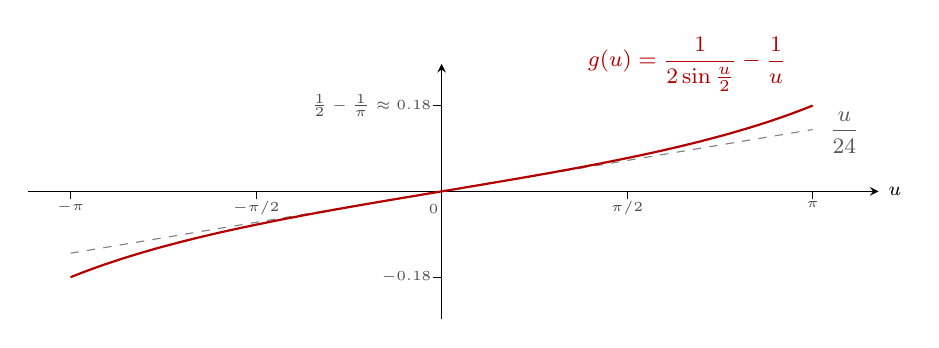
\begin{tikzpicture}[x=1.5cm,y=6cm]
  \taxes[u]{-3.5}{3.7}{0.27}{-0.27}
  \draw[gray,dashed,domain=-3.1416:3.1416] plot (\x,{\x/24});
  \draw[res] plot coordinates {(-3.1416,-0.1817) (-3.1102,-0.1785) (-3.0788,-0.1754) (-3.0473,-0.1724) (-3.0159,-0.1694) (-2.9845,-0.1665) (-2.9531,-0.1636) (-2.9217,-0.1608) (-2.8903,-0.1580) (-2.8588,-0.1552) (-2.8274,-0.1526) (-2.7960,-0.1499) (-2.7646,-0.1473) (-2.7332,-0.1447) (-2.7018,-0.1422) (-2.6704,-0.1397) (-2.6389,-0.1373) (-2.6075,-0.1349) (-2.5761,-0.1325) (-2.5447,-0.1302) (-2.5133,-0.1278) (-2.4819,-0.1256) (-2.4504,-0.1233) (-2.4190,-0.1211) (-2.3876,-0.1189) (-2.3562,-0.1168) (-2.3248,-0.1147) (-2.2934,-0.1126) (-2.2619,-0.1105) (-2.2305,-0.1085) (-2.1991,-0.1064) (-2.1677,-0.1044) (-2.1363,-0.1025) (-2.1049,-0.1005) (-2.0735,-0.0986) (-2.0420,-0.0967) (-2.0106,-0.0948) (-1.9792,-0.0930) (-1.9478,-0.0911) (-1.9164,-0.0893) (-1.8850,-0.0875) (-1.8535,-0.0857) (-1.8221,-0.0840) (-1.7907,-0.0822) (-1.7593,-0.0805) (-1.7279,-0.0788) (-1.6965,-0.0771) (-1.6650,-0.0754) (-1.6336,-0.0738) (-1.6022,-0.0721) (-1.5708,-0.0705) (-1.5394,-0.0689) (-1.5080,-0.0673) (-1.4765,-0.0657) (-1.4451,-0.0641) (-1.4137,-0.0625) (-1.3823,-0.0610) (-1.3509,-0.0594) (-1.3195,-0.0579) (-1.2881,-0.0564) (-1.2566,-0.0549) (-1.2252,-0.0534) (-1.1938,-0.0519) (-1.1624,-0.0504) (-1.1310,-0.0489) (-1.0996,-0.0475) (-1.0681,-0.0460) (-1.0367,-0.0446) (-1.0053,-0.0432) (-0.9739,-0.0417) (-0.9425,-0.0403) (-0.9111,-0.0389) (-0.8796,-0.0375) (-0.8482,-0.0361) (-0.8168,-0.0347) (-0.7854,-0.0333) (-0.7540,-0.0319) (-0.7226,-0.0306) (-0.6912,-0.0292) (-0.6597,-0.0278) (-0.6283,-0.0265) (-0.5969,-0.0251) (-0.5655,-0.0238) (-0.5341,-0.0224) (-0.5027,-0.0211) (-0.4712,-0.0198) (-0.4398,-0.0184) (-0.4084,-0.0171) (-0.3770,-0.0158) (-0.3456,-0.0144) (-0.3142,-0.0131) (-0.2827,-0.0118) (-0.2513,-0.0105) (-0.2199,-0.0092) (-0.1885,-0.0079) (-0.1571,-0.0065) (-0.1257,-0.0052) (-0.0942,-0.0039) (-0.0628,-0.0026) (-0.0314,-0.0013) (0.0000,0.0000) (0.0314,0.0013) (0.0628,0.0026) (0.0942,0.0039) (0.1257,0.0052) (0.1571,0.0065) (0.1885,0.0079) (0.2199,0.0092) (0.2513,0.0105) (0.2827,0.0118) (0.3142,0.0131) (0.3456,0.0144) (0.3770,0.0158) (0.4084,0.0171) (0.4398,0.0184) (0.4712,0.0198) (0.5027,0.0211) (0.5341,0.0224) (0.5655,0.0238) (0.5969,0.0251) (0.6283,0.0265) (0.6597,0.0278) (0.6912,0.0292) (0.7226,0.0306) (0.7540,0.0319) (0.7854,0.0333) (0.8168,0.0347) (0.8482,0.0361) (0.8796,0.0375) (0.9111,0.0389) (0.9425,0.0403) (0.9739,0.0417) (1.0053,0.0432) (1.0367,0.0446) (1.0681,0.0460) (1.0996,0.0475) (1.1310,0.0489) (1.1624,0.0504) (1.1938,0.0519) (1.2252,0.0534) (1.2566,0.0549) (1.2881,0.0564) (1.3195,0.0579) (1.3509,0.0594) (1.3823,0.0610) (1.4137,0.0625) (1.4451,0.0641) (1.4765,0.0657) (1.5080,0.0673) (1.5394,0.0689) (1.5708,0.0705) (1.6022,0.0721) (1.6336,0.0738) (1.6650,0.0754) (1.6965,0.0771) (1.7279,0.0788) (1.7593,0.0805) (1.7907,0.0822) (1.8221,0.0840) (1.8535,0.0857) (1.8850,0.0875) (1.9164,0.0893) (1.9478,0.0911) (1.9792,0.0930) (2.0106,0.0948) (2.0420,0.0967) (2.0735,0.0986) (2.1049,0.1005) (2.1363,0.1025) (2.1677,0.1044) (2.1991,0.1064) (2.2305,0.1085) (2.2619,0.1105) (2.2934,0.1126) (2.3248,0.1147) (2.3562,0.1168) (2.3876,0.1189) (2.4190,0.1211) (2.4504,0.1233) (2.4819,0.1256) (2.5133,0.1278) (2.5447,0.1302) (2.5761,0.1325) (2.6075,0.1349) (2.6389,0.1373) (2.6704,0.1397) (2.7018,0.1422) (2.7332,0.1447) (2.7646,0.1473) (2.7960,0.1499) (2.8274,0.1526) (2.8588,0.1552) (2.8903,0.1580) (2.9217,0.1608) (2.9531,0.1636) (2.9845,0.1665) (3.0159,0.1694) (3.0473,0.1724) (3.0788,0.1754) (3.1102,0.1785) (3.1416,0.1817)};
  % 纵轴放大了 6 倍，横轴刻度线用绝对长度，避免被拉长
  \draw (-3.1416,0) -- ++(0,-2.8pt) node[anchor=north,font=\tiny,gray!60!black,fill=white,inner sep=0.6pt] {$-\pi$};
  \draw (-1.5708,0) -- ++(0,-2.8pt) node[anchor=north,font=\tiny,gray!60!black,fill=white,inner sep=0.6pt] {$-\pi/2$};
  \draw (1.5708,0) -- ++(0,-2.8pt) node[anchor=north,font=\tiny,gray!60!black,fill=white,inner sep=0.6pt] {$\pi/2$};
  \draw (3.1416,0) -- ++(0,-2.8pt) node[anchor=north,font=\tiny,gray!60!black,fill=white,inner sep=0.6pt] {$\pi$};
  \draw (0,0.1817) -- (-0.07,0.1817) node[anchor=east,font=\tiny,gray!60!black,fill=white,inner sep=0.6pt] {$\frac12-\frac1\pi\approx0.18$};
  \draw (0,-0.1817) -- (-0.07,-0.1817) node[anchor=east,font=\tiny,gray!60!black,fill=white,inner sep=0.6pt] {$-0.18$};
  \node[font=\footnotesize,red!70!black,anchor=south east] at (3.0,0.19) {$g(u)=\dfrac{1}{2\sin\frac u2}-\dfrac1u$};
  \node[font=\footnotesize,gray!70!black,anchor=west] at (3.2,0.125) {$\dfrac{u}{24}$};
\end{tikzpicture}
\caption{$g(u)$ 在 $[-\pi,\pi]$ 上的形状（红）。它在 $u=0$ 处平滑地经过 $0$，附近与 $\frac{u}{24}$（灰虚线）重合；整个区间上 $|g(u)|\le\frac12-\frac1\pi\approx0.18$，没有无限上冲。}
\end{figure}

\point{结论。}补充定义 $g(0)=0$。这样 $g(u)$ 在 $[-\pi,\pi]$ 上不论 $u=0$ 还是 $u\ne0$，都有确定的有限值，并且处处可导、有界。于是把第一项中方括号外的部分整个看成一个函数
\[
y(u)=x\Big(\frac{u}{\omega_0}+t\Big)\,g(u)
\]
它满足狄利克雷三条件：$|y(u)|\le0.19\,\big|x\big(\frac{u}{\omega_0}+t\big)\big|$，仍绝对可积；$g(u)$ 单调、处处可导，相乘不会产生无穷多个极值或新的不连续点。$y(u)$ 乘以无限快的振荡 $\sin\big((N+\frac12)u\big)$ 后在一个周期上积分，由引理一，
\[
\lim_{N\to+\infty}\frac{1}{\pi}\int_{-\pi}^{\pi}y(u)\sin\!\Big(\big(N+\tfrac12\big)u\Big)\,\mathrm{d}u=0 .
\]
第一项的极限为 $0$。

\subsection{第七步：第二项用引理三}
在引理三中取 $\omega=N+\frac12$（$N\to+\infty$ 时 $\omega\to+\infty$），并把变量 $t$ 换成 $u$：
\[
\lim_{N\to+\infty}\frac{\sin\big((N+\frac12)u\big)}{u}=\pi\,\delta(u).
\]
代入第二项：
\[
\lim_{N\to+\infty}\frac{1}{\pi}\int_{-\pi}^{\pi}x\Big(\frac{u}{\omega_0}+t\Big)\frac{\sin\big((N+\frac12)u\big)}{u}\,\mathrm{d}u
=\frac1\pi\int_{-\pi}^{\pi}x\Big(\frac{u}{\omega_0}+t\Big)\,\pi\,\delta(u)\,\mathrm{d}u
=\int_{-\pi}^{\pi}x\Big(\frac{u}{\omega_0}+t\Big)\,\delta(u)\,\mathrm{d}u .
\]
积分区间 $[-\pi,\pi]$ 包含 $u=0$，由冲激函数的筛选性质 $\int f(u)\,\delta(u)\,\mathrm{d}u=f(0)$，结果是被积函数在 $u=0$ 的值：
\[
x\Big(\frac{0}{\omega_0}+t\Big)=x(t).
\]

\needspace{16\baselineskip}
\subsection{结论}
\begin{remember}
第一项 $\to0$，第二项 $\to x(t)$，所以
\[
\lim_{N\to+\infty}X_N(t)=0+x(t)=x(t).
\]
证明的主线：
\begin{enumerate}[nosep]
\item 代入系数、积化和差，$X_N(t)$ 变成 $x$ 与狄利克雷核 $D_N(u)=\frac{\sin((N+\frac12)u)}{2\sin(u/2)}$ 相乘再积分；
\item $D_N(u)$ 在 $u=0$ 处有奇点，用「减 $\frac1u$ 再加 $\frac1u$」拆成两项；
\item 去掉奇点的一项，由引理一（黎曼--勒贝格）趋于 $0$；
\item $\frac{\sin((N+\frac12)u)}{u}$ 一项趋于 $\pi\delta(u)$，由筛选性质取出 $x(t)$。
\end{enumerate}
\end{remember}

前面几步（代入系数、积化和差、换元、利用周期性）是常规运算；证明的关键在后面：用「减一项再加一项」去掉奇点，再把 $\frac{\sin((N+\frac12)u)}{u}$ 当成 $\pi\delta(u)$ 用。后者正是 $\delta$ 函数「又高又窄、面积不变」的思想。狄利克雷当年没有 $\delta$ 这个记号（它由狄拉克(Dirac)在 20 世纪 20 年代末引入），他是直接对积分取极限论证的；但这个证明里已经有了 $\delta$ 函数思想的雏形。

%==================================================================
\section{证明中的细节与数值验证}\label{sec:detail}

\subsection{不连续点处收敛到左右极限的平均值}\label{sub:jump}
第七步默认 $x\big(\frac{u}{\omega_0}+t\big)$ 在 $u=0$ 处连续，即 $x$ 在 $t$ 处连续。若 $t$ 是不连续点，$u>0$ 一侧取到的是右极限 $x(t^+)$，$u<0$ 一侧取到的是左极限 $x(t^-)$。$\frac{\sin(\omega u)}{u}$ 是偶函数，由引理二，两侧的面积各占一半：
\[
\int_0^{+\infty}\frac{\sin(\omega u)}{u}\,\mathrm{d}u=\int_{-\infty}^{0}\frac{\sin(\omega u)}{u}\,\mathrm{d}u=\frac{\pi}{2}.
\]
所以第二项的极限是 $\frac1\pi\big(\frac\pi2x(t^+)+\frac\pi2x(t^-)\big)$：
\begin{remember}
在不连续点处，
\[
\lim_{N\to+\infty}X_N(t)=\frac{x(t^+)+x(t^-)}{2}.
\]
\end{remember}

\subsection{三个条件分别用在哪里}
\begin{itemize}[nosep]
\item 条件 \textcircled{\scriptsize 1}（绝对可积）：保证系数积分存在，并保证第六步能用引理一。
\item 条件 \textcircled{\scriptsize 2}\textcircled{\scriptsize 3}（极值个数有限、不连续点个数有限）：第七步把 $\frac{\sin((N+\frac12)u)}{u}$ 当成 $\pi\delta(u)$ 用，需要 $x$ 在 $t$ 附近足够「规矩」——左右极限存在、附近不剧烈振荡。上面的证明直接借用了 $\delta$ 的筛选性质，没有展开这一点；严格的证明正是在这一步用到这两个条件。
\end{itemize}
这两个条件不是多余的：1873 年杜布瓦-雷蒙(du Bois-Reymond)构造出一个连续的周期函数，它的傅里叶级数在某一点发散。连续函数满足 \textcircled{\scriptsize 1}\textcircled{\scriptsize 3}，但它在一个周期内有无穷多个极值，不满足 \textcircled{\scriptsize 2}。

另一方面，狄利克雷条件只是\textbf{充分条件}：不满足它、傅里叶级数却仍收敛的函数也存在。

\subsection{数值验证：锯齿波}
\example{锯齿波的部分和}{连续点处 $\to x(t)$，跳变点处恒为 $\frac12$}{}
取周期 $T_0=2\pi$（$\omega_0=1$）的锯齿波：在 $[0,2\pi)$ 上 $x(t)=\frac{t}{2\pi}$，然后周期延拓。它满足狄利克雷条件：绝对可积，一个周期内单调（没有内部极值），只有一个跳变点（$t=0$ 处从 $1$ 跳到 $0$）。

\point{系数。}$B_0=\frac{1}{2\pi}\int_0^{2\pi}\frac{t}{2\pi}\,\mathrm{d}t=\frac12$。$x(t)-\frac12$ 是奇函数，所以 $B_k=0$。分部积分得
\[
C_k=\frac{1}{\pi}\int_0^{2\pi}\frac{t}{2\pi}\sin(kt)\,\mathrm{d}t=-\frac{1}{k\pi}.
\]
于是
\[
X_N(t)=\frac12-\sum_{k=1}^{N}\frac{\sin(kt)}{k\pi}.
\]

\point{连续点 $t=\frac\pi2$。}$x(\frac\pi2)=\frac14=0.25$。
\begin{center}
\begin{tabular}{cccccc}
\toprule
$N$ & $1$ & $10$ & $100$ & $1000$ & $10000$\\
\midrule
$X_N(\pi/2)$ & $0.1817$ & $0.2342$ & $0.25159$ & $0.250159$ & $0.2500159$\\
\bottomrule
\end{tabular}
\end{center}
误差随 $N$ 增大趋于 $0$，收敛到 $x(\frac\pi2)=0.25$。

\point{跳变点 $t=0$。}所有 $\sin(k\cdot0)=0$，$X_N(0)=\frac12$ 对每个 $N$ 都成立，正是左极限 $x(0^-)=1$ 与右极限 $x(0^+)=0$ 的平均值，与第 \ref{sub:jump} 节一致。

\begin{figure}[H]
\centering
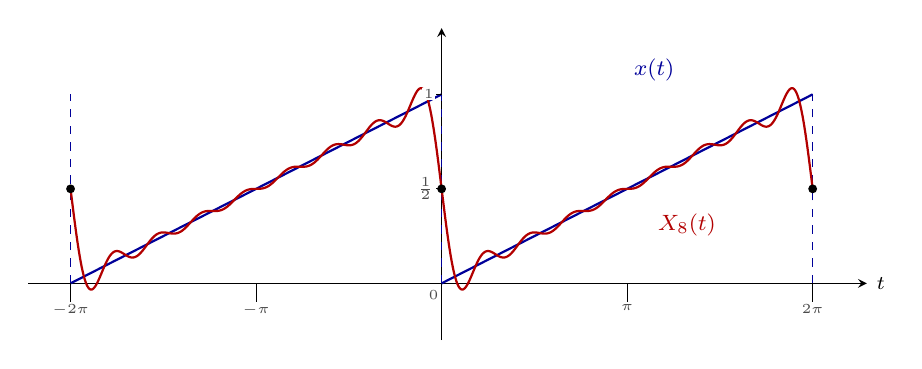
\begin{tikzpicture}[x=0.75cm,y=2.4cm]
  \taxes{-7}{7.2}{1.35}{-0.3}
  \draw[sig] (-6.2832,0) -- (0,1);
  \draw[sig] (0,0) -- (6.2832,1);
  \draw[sig,dashed,thin] (0,0) -- (0,1);
  \draw[sig,dashed,thin] (6.2832,0) -- (6.2832,1);
  \draw[sig,dashed,thin] (-6.2832,0) -- (-6.2832,1);
  \draw[res] plot coordinates {(-6.2832,0.5000) (-6.2675,0.4600) (-6.2518,0.4203) (-6.2361,0.3811) (-6.2204,0.3427) (-6.2046,0.3052) (-6.1889,0.2689) (-6.1732,0.2340) (-6.1575,0.2008) (-6.1418,0.1693) (-6.1261,0.1398) (-6.1104,0.1124) (-6.0947,0.0872) (-6.0790,0.0643) (-6.0633,0.0438) (-6.0476,0.0258) (-6.0319,0.0102) (-6.0161,-0.0029) (-6.0004,-0.0136) (-5.9847,-0.0218) (-5.9690,-0.0277) (-5.9533,-0.0314) (-5.9376,-0.0329) (-5.9219,-0.0323) (-5.9062,-0.0299) (-5.8905,-0.0257) (-5.8748,-0.0199) (-5.8591,-0.0128) (-5.8434,-0.0044) (-5.8277,0.0051) (-5.8119,0.0153) (-5.7962,0.0263) (-5.7805,0.0377) (-5.7648,0.0494) (-5.7491,0.0612) (-5.7334,0.0730) (-5.7177,0.0846) (-5.7020,0.0958) (-5.6863,0.1066) (-5.6706,0.1167) (-5.6549,0.1261) (-5.6392,0.1348) (-5.6235,0.1425) (-5.6077,0.1494) (-5.5920,0.1553) (-5.5763,0.1603) (-5.5606,0.1642) (-5.5449,0.1673) (-5.5292,0.1694) (-5.5135,0.1706) (-5.4978,0.1710) (-5.4821,0.1706) (-5.4664,0.1695) (-5.4507,0.1679) (-5.4350,0.1658) (-5.4192,0.1632) (-5.4035,0.1604) (-5.3878,0.1573) (-5.3721,0.1542) (-5.3564,0.1511) (-5.3407,0.1481) (-5.3250,0.1452) (-5.3093,0.1427) (-5.2936,0.1405) (-5.2779,0.1388) (-5.2622,0.1375) (-5.2465,0.1368) (-5.2308,0.1367) (-5.2150,0.1373) (-5.1993,0.1384) (-5.1836,0.1402) (-5.1679,0.1427) (-5.1522,0.1457) (-5.1365,0.1494) (-5.1208,0.1536) (-5.1051,0.1584) (-5.0894,0.1636) (-5.0737,0.1693) (-5.0580,0.1752) (-5.0423,0.1815) (-5.0265,0.1880) (-5.0108,0.1946) (-4.9951,0.2012) (-4.9794,0.2079) (-4.9637,0.2144) (-4.9480,0.2208) (-4.9323,0.2270) (-4.9166,0.2329) (-4.9009,0.2384) (-4.8852,0.2436) (-4.8695,0.2483) (-4.8538,0.2526) (-4.8381,0.2564) (-4.8223,0.2597) (-4.8066,0.2625) (-4.7909,0.2648) (-4.7752,0.2666) (-4.7595,0.2680) (-4.7438,0.2689) (-4.7281,0.2694) (-4.7124,0.2696) (-4.6967,0.2695) (-4.6810,0.2690) (-4.6653,0.2684) (-4.6496,0.2677) (-4.6338,0.2668) (-4.6181,0.2659) (-4.6024,0.2651) (-4.5867,0.2643) (-4.5710,0.2637) (-4.5553,0.2633) (-4.5396,0.2631) (-4.5239,0.2632) (-4.5082,0.2637) (-4.4925,0.2645) (-4.4768,0.2657) (-4.4611,0.2673) (-4.4454,0.2693) (-4.4296,0.2717) (-4.4139,0.2746) (-4.3982,0.2778) (-4.3825,0.2815) (-4.3668,0.2855) (-4.3511,0.2898) (-4.3354,0.2945) (-4.3197,0.2994) (-4.3040,0.3044) (-4.2883,0.3097) (-4.2726,0.3151) (-4.2569,0.3205) (-4.2412,0.3259) (-4.2254,0.3313) (-4.2097,0.3366) (-4.1940,0.3418) (-4.1783,0.3467) (-4.1626,0.3515) (-4.1469,0.3559) (-4.1312,0.3601) (-4.1155,0.3639) (-4.0998,0.3674) (-4.0841,0.3706) (-4.0684,0.3733) (-4.0527,0.3757) (-4.0369,0.3777) (-4.0212,0.3794) (-4.0055,0.3807) (-3.9898,0.3817) (-3.9741,0.3824) (-3.9584,0.3828) (-3.9427,0.3831) (-3.9270,0.3832) (-3.9113,0.3831) (-3.8956,0.3830) (-3.8799,0.3828) (-3.8642,0.3826) (-3.8485,0.3825) (-3.8327,0.3825) (-3.8170,0.3827) (-3.8013,0.3830) (-3.7856,0.3835) (-3.7699,0.3844) (-3.7542,0.3855) (-3.7385,0.3869) (-3.7228,0.3886) (-3.7071,0.3907) (-3.6914,0.3931) (-3.6757,0.3959) (-3.6600,0.3990) (-3.6442,0.4025) (-3.6285,0.4062) (-3.6128,0.4102) (-3.5971,0.4145) (-3.5814,0.4191) (-3.5657,0.4238) (-3.5500,0.4286) (-3.5343,0.4336) (-3.5186,0.4386) (-3.5029,0.4436) (-3.4872,0.4487) (-3.4715,0.4536) (-3.4558,0.4584) (-3.4400,0.4631) (-3.4243,0.4676) (-3.4086,0.4718) (-3.3929,0.4758) (-3.3772,0.4795) (-3.3615,0.4829) (-3.3458,0.4860) (-3.3301,0.4887) (-3.3144,0.4911) (-3.2987,0.4932) (-3.2830,0.4950) (-3.2673,0.4964) (-3.2515,0.4976) (-3.2358,0.4985) (-3.2201,0.4991) (-3.2044,0.4995) (-3.1887,0.4998) (-3.1730,0.4999) (-3.1573,0.5000) (-3.1416,0.5000) (-3.1259,0.5000) (-3.1102,0.5001) (-3.0945,0.5002) (-3.0788,0.5005) (-3.0631,0.5009) (-3.0473,0.5015) (-3.0316,0.5024) (-3.0159,0.5036) (-3.0002,0.5050) (-2.9845,0.5068) (-2.9688,0.5089) (-2.9531,0.5113) (-2.9374,0.5140) (-2.9217,0.5171) (-2.9060,0.5205) (-2.8903,0.5242) (-2.8746,0.5282) (-2.8588,0.5324) (-2.8431,0.5369) (-2.8274,0.5416) (-2.8117,0.5464) (-2.7960,0.5513) (-2.7803,0.5564) (-2.7646,0.5614) (-2.7489,0.5664) (-2.7332,0.5714) (-2.7175,0.5762) (-2.7018,0.5809) (-2.6861,0.5855) (-2.6704,0.5898) (-2.6546,0.5938) (-2.6389,0.5975) (-2.6232,0.6010) (-2.6075,0.6041) (-2.5918,0.6069) (-2.5761,0.6093) (-2.5604,0.6114) (-2.5447,0.6131) (-2.5290,0.6145) (-2.5133,0.6156) (-2.4976,0.6165) (-2.4819,0.6170) (-2.4662,0.6173) (-2.4504,0.6175) (-2.4347,0.6175) (-2.4190,0.6174) (-2.4033,0.6172) (-2.3876,0.6170) (-2.3719,0.6169) (-2.3562,0.6168) (-2.3405,0.6169) (-2.3248,0.6172) (-2.3091,0.6176) (-2.2934,0.6183) (-2.2777,0.6193) (-2.2619,0.6206) (-2.2462,0.6223) (-2.2305,0.6243) (-2.2148,0.6267) (-2.1991,0.6294) (-2.1834,0.6326) (-2.1677,0.6361) (-2.1520,0.6399) (-2.1363,0.6441) (-2.1206,0.6485) (-2.1049,0.6533) (-2.0892,0.6582) (-2.0735,0.6634) (-2.0577,0.6687) (-2.0420,0.6741) (-2.0263,0.6795) (-2.0106,0.6849) (-1.9949,0.6903) (-1.9792,0.6956) (-1.9635,0.7006) (-1.9478,0.7055) (-1.9321,0.7102) (-1.9164,0.7145) (-1.9007,0.7185) (-1.8850,0.7222) (-1.8692,0.7254) (-1.8535,0.7283) (-1.8378,0.7307) (-1.8221,0.7327) (-1.8064,0.7343) (-1.7907,0.7355) (-1.7750,0.7363) (-1.7593,0.7368) (-1.7436,0.7369) (-1.7279,0.7367) (-1.7122,0.7363) (-1.6965,0.7357) (-1.6808,0.7349) (-1.6650,0.7341) (-1.6493,0.7332) (-1.6336,0.7323) (-1.6179,0.7316) (-1.6022,0.7310) (-1.5865,0.7305) (-1.5708,0.7304) (-1.5551,0.7306) (-1.5394,0.7311) (-1.5237,0.7320) (-1.5080,0.7334) (-1.4923,0.7352) (-1.4765,0.7375) (-1.4608,0.7403) (-1.4451,0.7436) (-1.4294,0.7474) (-1.4137,0.7517) (-1.3980,0.7564) (-1.3823,0.7616) (-1.3666,0.7671) (-1.3509,0.7730) (-1.3352,0.7792) (-1.3195,0.7856) (-1.3038,0.7921) (-1.2881,0.7988) (-1.2723,0.8054) (-1.2566,0.8120) (-1.2409,0.8185) (-1.2252,0.8248) (-1.2095,0.8307) (-1.1938,0.8364) (-1.1781,0.8416) (-1.1624,0.8464) (-1.1467,0.8506) (-1.1310,0.8543) (-1.1153,0.8573) (-1.0996,0.8598) (-1.0838,0.8616) (-1.0681,0.8627) (-1.0524,0.8633) (-1.0367,0.8632) (-1.0210,0.8625) (-1.0053,0.8612) (-0.9896,0.8595) (-0.9739,0.8573) (-0.9582,0.8548) (-0.9425,0.8519) (-0.9268,0.8489) (-0.9111,0.8458) (-0.8954,0.8427) (-0.8796,0.8396) (-0.8639,0.8368) (-0.8482,0.8342) (-0.8325,0.8321) (-0.8168,0.8305) (-0.8011,0.8294) (-0.7854,0.8290) (-0.7697,0.8294) (-0.7540,0.8306) (-0.7383,0.8327) (-0.7226,0.8358) (-0.7069,0.8397) (-0.6912,0.8447) (-0.6754,0.8506) (-0.6597,0.8575) (-0.6440,0.8652) (-0.6283,0.8739) (-0.6126,0.8833) (-0.5969,0.8934) (-0.5812,0.9042) (-0.5655,0.9154) (-0.5498,0.9270) (-0.5341,0.9388) (-0.5184,0.9506) (-0.5027,0.9623) (-0.4869,0.9737) (-0.4712,0.9847) (-0.4555,0.9949) (-0.4398,1.0044) (-0.4241,1.0128) (-0.4084,1.0199) (-0.3927,1.0257) (-0.3770,1.0299) (-0.3613,1.0323) (-0.3456,1.0329) (-0.3299,1.0314) (-0.3142,1.0277) (-0.2985,1.0218) (-0.2827,1.0136) (-0.2670,1.0029) (-0.2513,0.9898) (-0.2356,0.9742) (-0.2199,0.9562) (-0.2042,0.9357) (-0.1885,0.9128) (-0.1728,0.8876) (-0.1571,0.8602) (-0.1414,0.8307) (-0.1257,0.7992) (-0.1100,0.7660) (-0.0942,0.7311) (-0.0785,0.6948) (-0.0628,0.6573) (-0.0471,0.6189) (-0.0314,0.5797) (-0.0157,0.5400) (0.0000,0.5000) (0.0157,0.4600) (0.0314,0.4203) (0.0471,0.3811) (0.0628,0.3427) (0.0785,0.3052) (0.0942,0.2689) (0.1100,0.2340) (0.1257,0.2008) (0.1414,0.1693) (0.1571,0.1398) (0.1728,0.1124) (0.1885,0.0872) (0.2042,0.0643) (0.2199,0.0438) (0.2356,0.0258) (0.2513,0.0102) (0.2670,-0.0029) (0.2827,-0.0136) (0.2985,-0.0218) (0.3142,-0.0277) (0.3299,-0.0314) (0.3456,-0.0329) (0.3613,-0.0323) (0.3770,-0.0299) (0.3927,-0.0257) (0.4084,-0.0199) (0.4241,-0.0128) (0.4398,-0.0044) (0.4555,0.0051) (0.4712,0.0153) (0.4869,0.0263) (0.5027,0.0377) (0.5184,0.0494) (0.5341,0.0612) (0.5498,0.0730) (0.5655,0.0846) (0.5812,0.0958) (0.5969,0.1066) (0.6126,0.1167) (0.6283,0.1261) (0.6440,0.1348) (0.6597,0.1425) (0.6754,0.1494) (0.6912,0.1553) (0.7069,0.1603) (0.7226,0.1642) (0.7383,0.1673) (0.7540,0.1694) (0.7697,0.1706) (0.7854,0.1710) (0.8011,0.1706) (0.8168,0.1695) (0.8325,0.1679) (0.8482,0.1658) (0.8639,0.1632) (0.8796,0.1604) (0.8954,0.1573) (0.9111,0.1542) (0.9268,0.1511) (0.9425,0.1481) (0.9582,0.1452) (0.9739,0.1427) (0.9896,0.1405) (1.0053,0.1388) (1.0210,0.1375) (1.0367,0.1368) (1.0524,0.1367) (1.0681,0.1373) (1.0838,0.1384) (1.0996,0.1402) (1.1153,0.1427) (1.1310,0.1457) (1.1467,0.1494) (1.1624,0.1536) (1.1781,0.1584) (1.1938,0.1636) (1.2095,0.1693) (1.2252,0.1752) (1.2409,0.1815) (1.2566,0.1880) (1.2723,0.1946) (1.2881,0.2012) (1.3038,0.2079) (1.3195,0.2144) (1.3352,0.2208) (1.3509,0.2270) (1.3666,0.2329) (1.3823,0.2384) (1.3980,0.2436) (1.4137,0.2483) (1.4294,0.2526) (1.4451,0.2564) (1.4608,0.2597) (1.4765,0.2625) (1.4923,0.2648) (1.5080,0.2666) (1.5237,0.2680) (1.5394,0.2689) (1.5551,0.2694) (1.5708,0.2696) (1.5865,0.2695) (1.6022,0.2690) (1.6179,0.2684) (1.6336,0.2677) (1.6493,0.2668) (1.6650,0.2659) (1.6808,0.2651) (1.6965,0.2643) (1.7122,0.2637) (1.7279,0.2633) (1.7436,0.2631) (1.7593,0.2632) (1.7750,0.2637) (1.7907,0.2645) (1.8064,0.2657) (1.8221,0.2673) (1.8378,0.2693) (1.8535,0.2717) (1.8692,0.2746) (1.8850,0.2778) (1.9007,0.2815) (1.9164,0.2855) (1.9321,0.2898) (1.9478,0.2945) (1.9635,0.2994) (1.9792,0.3044) (1.9949,0.3097) (2.0106,0.3151) (2.0263,0.3205) (2.0420,0.3259) (2.0577,0.3313) (2.0735,0.3366) (2.0892,0.3418) (2.1049,0.3467) (2.1206,0.3515) (2.1363,0.3559) (2.1520,0.3601) (2.1677,0.3639) (2.1834,0.3674) (2.1991,0.3706) (2.2148,0.3733) (2.2305,0.3757) (2.2462,0.3777) (2.2619,0.3794) (2.2777,0.3807) (2.2934,0.3817) (2.3091,0.3824) (2.3248,0.3828) (2.3405,0.3831) (2.3562,0.3832) (2.3719,0.3831) (2.3876,0.3830) (2.4033,0.3828) (2.4190,0.3826) (2.4347,0.3825) (2.4504,0.3825) (2.4662,0.3827) (2.4819,0.3830) (2.4976,0.3835) (2.5133,0.3844) (2.5290,0.3855) (2.5447,0.3869) (2.5604,0.3886) (2.5761,0.3907) (2.5918,0.3931) (2.6075,0.3959) (2.6232,0.3990) (2.6389,0.4025) (2.6546,0.4062) (2.6704,0.4102) (2.6861,0.4145) (2.7018,0.4191) (2.7175,0.4238) (2.7332,0.4286) (2.7489,0.4336) (2.7646,0.4386) (2.7803,0.4436) (2.7960,0.4487) (2.8117,0.4536) (2.8274,0.4584) (2.8431,0.4631) (2.8588,0.4676) (2.8746,0.4718) (2.8903,0.4758) (2.9060,0.4795) (2.9217,0.4829) (2.9374,0.4860) (2.9531,0.4887) (2.9688,0.4911) (2.9845,0.4932) (3.0002,0.4950) (3.0159,0.4964) (3.0316,0.4976) (3.0473,0.4985) (3.0631,0.4991) (3.0788,0.4995) (3.0945,0.4998) (3.1102,0.4999) (3.1259,0.5000) (3.1416,0.5000) (3.1573,0.5000) (3.1730,0.5001) (3.1887,0.5002) (3.2044,0.5005) (3.2201,0.5009) (3.2358,0.5015) (3.2515,0.5024) (3.2673,0.5036) (3.2830,0.5050) (3.2987,0.5068) (3.3144,0.5089) (3.3301,0.5113) (3.3458,0.5140) (3.3615,0.5171) (3.3772,0.5205) (3.3929,0.5242) (3.4086,0.5282) (3.4243,0.5324) (3.4400,0.5369) (3.4558,0.5416) (3.4715,0.5464) (3.4872,0.5513) (3.5029,0.5564) (3.5186,0.5614) (3.5343,0.5664) (3.5500,0.5714) (3.5657,0.5762) (3.5814,0.5809) (3.5971,0.5855) (3.6128,0.5898) (3.6285,0.5938) (3.6442,0.5975) (3.6600,0.6010) (3.6757,0.6041) (3.6914,0.6069) (3.7071,0.6093) (3.7228,0.6114) (3.7385,0.6131) (3.7542,0.6145) (3.7699,0.6156) (3.7856,0.6165) (3.8013,0.6170) (3.8170,0.6173) (3.8327,0.6175) (3.8485,0.6175) (3.8642,0.6174) (3.8799,0.6172) (3.8956,0.6170) (3.9113,0.6169) (3.9270,0.6168) (3.9427,0.6169) (3.9584,0.6172) (3.9741,0.6176) (3.9898,0.6183) (4.0055,0.6193) (4.0212,0.6206) (4.0369,0.6223) (4.0527,0.6243) (4.0684,0.6267) (4.0841,0.6294) (4.0998,0.6326) (4.1155,0.6361) (4.1312,0.6399) (4.1469,0.6441) (4.1626,0.6485) (4.1783,0.6533) (4.1940,0.6582) (4.2097,0.6634) (4.2254,0.6687) (4.2412,0.6741) (4.2569,0.6795) (4.2726,0.6849) (4.2883,0.6903) (4.3040,0.6956) (4.3197,0.7006) (4.3354,0.7055) (4.3511,0.7102) (4.3668,0.7145) (4.3825,0.7185) (4.3982,0.7222) (4.4139,0.7254) (4.4296,0.7283) (4.4454,0.7307) (4.4611,0.7327) (4.4768,0.7343) (4.4925,0.7355) (4.5082,0.7363) (4.5239,0.7368) (4.5396,0.7369) (4.5553,0.7367) (4.5710,0.7363) (4.5867,0.7357) (4.6024,0.7349) (4.6181,0.7341) (4.6338,0.7332) (4.6496,0.7323) (4.6653,0.7316) (4.6810,0.7310) (4.6967,0.7305) (4.7124,0.7304) (4.7281,0.7306) (4.7438,0.7311) (4.7595,0.7320) (4.7752,0.7334) (4.7909,0.7352) (4.8066,0.7375) (4.8223,0.7403) (4.8381,0.7436) (4.8538,0.7474) (4.8695,0.7517) (4.8852,0.7564) (4.9009,0.7616) (4.9166,0.7671) (4.9323,0.7730) (4.9480,0.7792) (4.9637,0.7856) (4.9794,0.7921) (4.9951,0.7988) (5.0108,0.8054) (5.0265,0.8120) (5.0423,0.8185) (5.0580,0.8248) (5.0737,0.8307) (5.0894,0.8364) (5.1051,0.8416) (5.1208,0.8464) (5.1365,0.8506) (5.1522,0.8543) (5.1679,0.8573) (5.1836,0.8598) (5.1993,0.8616) (5.2150,0.8627) (5.2308,0.8633) (5.2465,0.8632) (5.2622,0.8625) (5.2779,0.8612) (5.2936,0.8595) (5.3093,0.8573) (5.3250,0.8548) (5.3407,0.8519) (5.3564,0.8489) (5.3721,0.8458) (5.3878,0.8427) (5.4035,0.8396) (5.4192,0.8368) (5.4350,0.8342) (5.4507,0.8321) (5.4664,0.8305) (5.4821,0.8294) (5.4978,0.8290) (5.5135,0.8294) (5.5292,0.8306) (5.5449,0.8327) (5.5606,0.8358) (5.5763,0.8397) (5.5920,0.8447) (5.6077,0.8506) (5.6235,0.8575) (5.6392,0.8652) (5.6549,0.8739) (5.6706,0.8833) (5.6863,0.8934) (5.7020,0.9042) (5.7177,0.9154) (5.7334,0.9270) (5.7491,0.9388) (5.7648,0.9506) (5.7805,0.9623) (5.7962,0.9737) (5.8119,0.9847) (5.8277,0.9949) (5.8434,1.0044) (5.8591,1.0128) (5.8748,1.0199) (5.8905,1.0257) (5.9062,1.0299) (5.9219,1.0323) (5.9376,1.0329) (5.9533,1.0314) (5.9690,1.0277) (5.9847,1.0218) (6.0004,1.0136) (6.0161,1.0029) (6.0319,0.9898) (6.0476,0.9742) (6.0633,0.9562) (6.0790,0.9357) (6.0947,0.9128) (6.1104,0.8876) (6.1261,0.8602) (6.1418,0.8307) (6.1575,0.7992) (6.1732,0.7660) (6.1889,0.7311) (6.2046,0.6948) (6.2204,0.6573) (6.2361,0.6189) (6.2518,0.5797) (6.2675,0.5400) (6.2832,0.5000)};
  \fill[black] (0,0.5) circle (1.6pt);
  \fill[black] (6.2832,0.5) circle (1.6pt);
  \fill[black] (-6.2832,0.5) circle (1.6pt);
  \xt{-6.2832}{-2\pi}\xt{-3.1416}{-\pi}\xt{3.1416}{\pi}\xt{6.2832}{2\pi}
  \yt{0.5}{\frac12}\yt{1}{1}
  \node[font=\footnotesize,blue!60!black,anchor=south] at (3.6,1.02) {$x(t)$};
  \node[font=\footnotesize,red!70!black,anchor=north west] at (3.5,0.42) {$X_8(t)$};
\end{tikzpicture}
\caption{锯齿波 $x(t)$（蓝）与部分和 $X_8(t)$（红）。连续处 $X_8(t)$ 已贴近 $x(t)$；在跳变点 $t=0,\pm2\pi$，部分和恒取左右极限的平均值 $\frac12$（黑点）。跳变点两侧的过冲就是吉布斯现象，$N$ 增大时它不会消失，只是越来越窄。}
\end{figure}

\end{document}
